\documentclass[12pt,oneside,a4paper]{book}

%%%%%%%%%%%%%%%%%%%%%%%%% preamble %%%%%%%%%%%%%%%%%%%%%%%%%
%% 引用宏包 %%
\usepackage{ctex}
\usepackage{titlesec}
\usepackage{amsmath,amssymb,amsthm,multicol,siunitx,graphicx,enumitem,booktabs,appendix}
\usepackage{booktabs}
\usepackage{tabularx,subcaption,arydshln}
\usepackage{tikz}
\usepackage{arydshln}
\usetikzlibrary{calc}
\usetikzlibrary{positioning}
\usetikzlibrary{matrix, positioning, arrows}
\usepackage[edges]{forest}
\usepackage{pgfplots}
\pgfplotsset{compat=1.8}
\usepackage{imakeidx}
\usepackage{framed}
\usepackage{makecell}
\usepackage{multirow}
\usepackage[export]{adjustbox}

%% 超链接与引用 %%
\usepackage{hyperref}
\hypersetup{
    hidelinks, % 取消红框
    colorlinks=true,
    linkcolor=blue,
    citecolor=pink
}
\renewcommand{\figureautorefname}{图}
\renewcommand{\tableautorefname}{表}
\renewcommand{\equationautorefname}{公式}
\def\chapterautorefname~#1\null{第~#1~章\null}
\def\sectionautorefname~#1\null{第~#1~节\null}
\def\subsectionautorefname~#1\null{第~#1~小节\null}


%%%%%%%%%%%%%%%%%%%%%%%%%%% info %%%%%%%%%%%%%%%%%%%%%%%%%%%

%% 文档信息及标题 %%
\title{凝聚态物理}
\author{}
\date{\today}


%%%%%%%%%%%%%%%%%%%%%%%%% document %%%%%%%%%%%%%%%%%%%%%%%%%
\begin{document}
\maketitle          %标题

\frontmatter
\chapter{前言}
\textbf{关于本书}

作为笔者对\textbf{凝聚态物理}的学习笔记,本书涵盖《固体物理》、《半导体物理》、《固态器件》三门学科。

在第一部分《固体物理》中,我们将介绍\textbf{固态晶体}的晶格结构、倒格子、晶格振动、能带理论等内容;

在第二部分《半导体物理》中,我们将介绍\textbf{半导体}的电子状态、掺杂与缺陷、载流子的统计分布、导电性、非平衡载流子等内容;

在第三部分《固态器件》中,我们将介绍PN结、肖特基二极管、双极性晶体管、异质结晶体管、MOS场效应管等\textbf{半导体器件}。

\hspace{2em}

\textbf{内容参考}

整理笔记过程中,参考了普渡大学\href{https://nanohub.org/courses/ECE606/2020x/outline}{ECE 606:固态器件}课程。

笔记亦可作为电子科学与技术专业学生的参考资料。

\hspace{2em}

\textbf{致谢}

由于笔者能力有限,内容势必存在不足与缺漏,敬请斧正。

\tableofcontents    %目录

\mainmatter

\part{固体物理}
\chapter{晶体结构与性质}
\section{常见晶体结构}
\subsection{凝聚态}
    \textbf{凝聚态}\index{凝聚态},指的是由大量粒子组成的、并且粒子间有很强的相互作用的系统,一般包括固体、液体以及介于二者之间的软物质(例如凝胶、液晶)。

    \textbf{固体}\index{固体}是凝聚态的一种特殊聚集形式。当压强与温度一定,且无外力作用时,固体的形状和体积保持不变——而液体则没有这种性质。固体由大量的原子(或离子)构成,每$1cm^3$体积中大约有$10^{23}$个粒子,大量粒子以一定的形式排列,我们将粒子排列的方式称为固体的结构。

    按照固体中粒子排列的有序度和对称性,固体可以分为晶体、非晶体和准晶体三类,如\autoref{fig:1-01}所示:
    \begin{itemize}[itemsep=0pt,parsep=0pt]
        \item \textbf{晶体}\index{晶体}:晶体中的组成粒子在空间周期性排列,称为长程序。
        \item \textbf{非晶体}\index{非晶体}:非晶体中的组成粒子在空间中不具备周期性,也并非完全无序,称为短程序。
        \item \textbf{准晶体}\index{准晶体}:准晶体介于晶体与非晶体之间。它的粒子分布是有序的,但不具备周期性,仅具备长程取向序。
    \end{itemize}
    具体来说,非晶体的排列是混乱无序的,或者说其规律仅适用于较小的空间内;而晶体与准晶体的排列则是有序规律的。然而,晶体可以无空隙地填充整个空间,准晶体同样可以填充空间,但不可避免的存在空隙。

    \begin{figure}[!htbp]
        \centering
        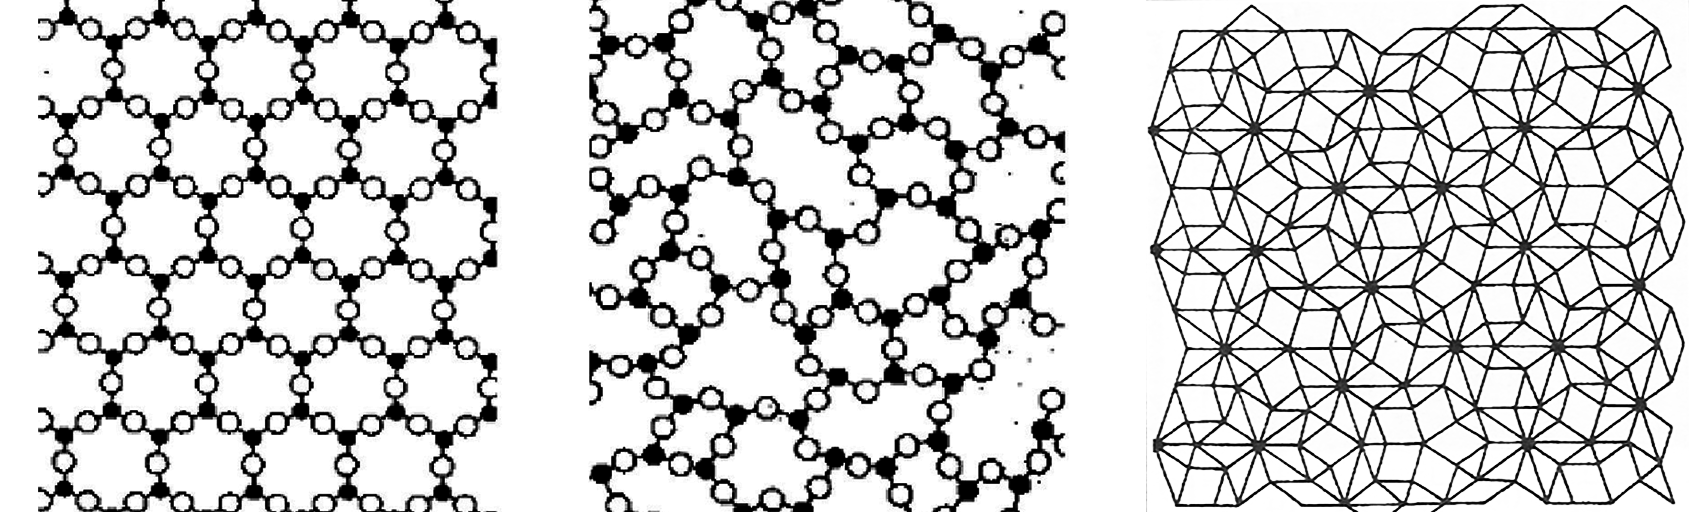
\includegraphics[width=\textwidth, keepaspectratio=true]{pic/1-01}
        \caption{晶体、非晶体与准晶体的粒子排列}
        \label{fig:1-01}
    \end{figure}

\subsection{晶格}
    晶体中,粒子排列的具体周期性结构称为\textbf{晶格}\index{晶格}。不同晶体具有不同的粒子排列结构,我们称为具有不同的晶格。
    
    我们在本节介绍若干种常见的晶体结构。为了便于理解,我们把晶格视为球体的堆积,即一个个原子呈球形,且彼此紧密的堆积在一起。

    \autoref{tab:1-1}引入下列晶格参数,从而方便地描述晶格特性:
    \begin{table}[!htbp]
        \centering
        \setlength{\tabcolsep}{1em}
        \begin{tabular}{lcl}
            \toprule
            晶格参数    &   字母表示    &   含义    \\
            \midrule
            晶格常数    &   $a$     &   标注某条棱的长度\\
            有效原子数  &           &   晶格内所含有的原子数\\
            配位数      &   $n$     &   与某原子距离最近的原子数\\
            最近邻距离  &           &   与某原子距离最近的原子的距离\\
            致密度      &   $\rho$  &   $\mbox{致密度}\rho=\frac{\mbox{有效原子数}\times \mbox{原子体积}}{\mbox{晶格体积}}$\\
            密排方向    &           &   在某个方向上原子密排\\
            \bottomrule
        \end{tabular}
        \caption{晶格常数}
        \label{tab:1-1}
    \end{table}

\newpage 
\subsubsection{第一类晶格:立方体结构}
    将同种粒子放在正方形的顶点上,即可得到平面的二维正方结构;\\
    同理我们推广到三维情况。所有的立方体结构晶格如\autoref{tab:1-2}所示。
    \begin{itemize}[itemsep=0pt,parsep=0pt]
        \item \textbf{简单立方}\index{简单立方}:将同种粒子放在立方体的顶点上,即为简单立方结构。\footnote{简单立方结构在自然界中极其罕见,目前唯一实例是钋($Po$)的$\alpha$相晶体}
        \item \textbf{面心立方}\index{面心立方}:在简单立方的基础上,若立方体面心还有一个粒子,即为面心立方结构。\footnote{应当指出,面心立方即为最密堆积的ABC结构。}
        \item \textbf{体心立方}\index{体心立方}:在简单立方的基础上,若立方体体心还有一个粒子,即为体心立方结构。
    \end{itemize}

    \begin{table}[!htbp]
        \centering
        \resizebox{\textwidth}{!}{
        \setlength{\tabcolsep}{1em}
        \begin{tabular}{ccccc}
                & 二维正方 & 简单立方 & 面心立方 & 体心立方\\
                & 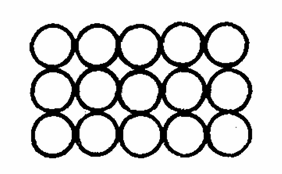
\includegraphics[height=6em, keepaspectratio=true]{pic/1-02} & 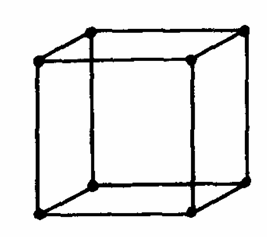
\includegraphics[height=6em, keepaspectratio=true]{pic/1-03} & 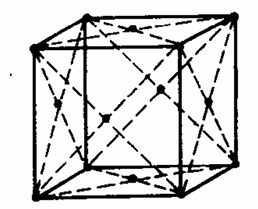
\includegraphics[height=6em, keepaspectratio=true]{pic/1-04} & 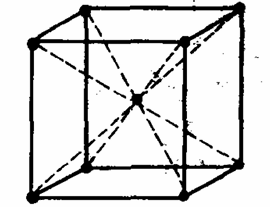
\includegraphics[height=6em, keepaspectratio=true]{pic/1-05}\\
            晶格常数$a$ & a & a & a & a \\
            密排方向    &沿边$a=2r$&沿棱$a=2r$&沿面对角线$\sqrt{2}a=4r$&沿体对角线$\sqrt{3}a=4r$\\
            有效原子数  &$4\times \frac{1}{4} = 1$&$8\times \frac{1}{8} = 1$&$8\times \frac{1}{8} + 6\times \frac{1}{2}= 4$&$8\times \frac{1}{8} + 1\times 1= 2$\\
            配位数$n$   &4&6&12&8\\
            最近邻距离  &$a$&$a$&$\frac{\sqrt{2}}{2}a$&$\frac{\sqrt{3}}{2}a$\\
            致密度$\rho$&&$\rho_1=\frac{1\times \frac{4}{3} \pi r^3}{(2r)^3} = \frac{\pi}{6}$&$\rho_2=\frac{4\times \frac{4}{3} \pi r^3}{(2\sqrt{2}r)^3} = \frac{\sqrt{2}}{6}\pi$&$\rho_3=\frac{2\times \frac{4}{3} \pi r^3}{(\frac{4}{\sqrt{3}}r)^3} = \frac{\sqrt{3}}{8}\pi$\\
        \end{tabular}
        }
        \caption{立方体结构晶格}
        \label{tab:1-2}
    \end{table}

\subsubsection{第二类晶格:密堆积结构}
    我们考虑这样的问题:如何排列,可以使得二维平面内可以放下最多的球体?这就是二维等径球最密堆积问题。可以证明,\autoref{fig:1-02}这样的排列是平面内的最密排列,称这种原子球在平面内最紧密排列的方式为\textbf{密排面}\index{密排面}。

    \begin{figure}[!htbp]
        \centering
        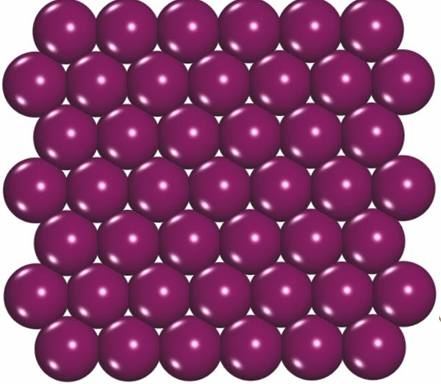
\includegraphics[height=8em, keepaspectratio=true]{pic/1-09}
        \caption{二维等径球最密堆积}
        \label{fig:1-02}
    \end{figure}

    仔细观察\autoref{fig:1-03}这样的密排面,我们应当注意到它具有两种不同的三角形空隙——一种三角形的尖尖朝上,如图中的第一排空隙B所示;另一种的三角形的尖尖朝下,如图中的第二排空隙C所示。两种空隙彼此交错。

    \begin{figure}[!htbp]
        \centering
        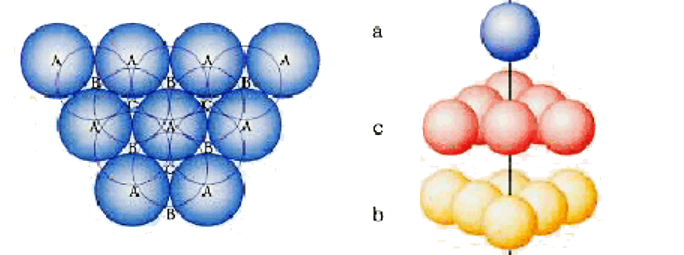
\includegraphics[height=8em, keepaspectratio=true]{pic/1-10}
        \caption{密排面的空隙}
        \label{fig:1-03}
    \end{figure}

    推广到三维情况,为了堆积得最紧密,由若干个这样的密排面一层层叠加起来,将一层的球心对准另一层的空隙。这就出现了两种堆叠方式,并由此形成了两种完全不同密堆积结构:AB型,与ABC型,如\autoref{fig:1-04}所示。
    
    顾名思义,第一种堆积方式即第一层的球心A对齐第二层的空隙B,并继续堆积第三层的球心A';第二种堆积方式则是第一层的球心先对齐第二层的空隙B,再对齐第三层的另一种空隙C,最后堆积新的一层的球心。
    
    \begin{figure}[!htbp]
        \centering
        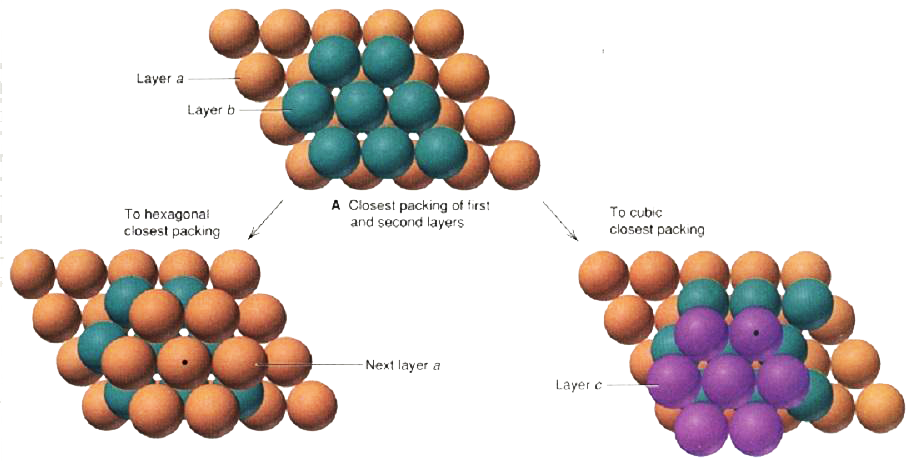
\includegraphics[height=12em, keepaspectratio=true]{pic/1-11}
        \caption{两种密堆积结构:AB型与ABC型}
        \label{fig:1-04}
    \end{figure}

    应当指出:ABC型堆积中,BC的顺序并不重要。根据观察的角度不同,空隙的指向也会变换,我们只要求BC两层空隙的角度相反。也可以认为,对于$\dots$\textcolor{red}{\textbf{ABC}}ABC$\dots$的堆积,我们从相反方向观察,就自然变成了$\dots$CB\textcolor{red}{\textbf{ACB}}A$\dots$的堆积。

    归纳密堆积结构晶格如\autoref{tab:1-3}所示:
    \begin{table}[!htbp]
        \centering
        \resizebox{\textwidth}{!}{
        \setlength{\tabcolsep}{1em}
        \begin{tabular}{cccc}
                & 二维六角 & 六角密排AB & 面心立方ABC\\
                & 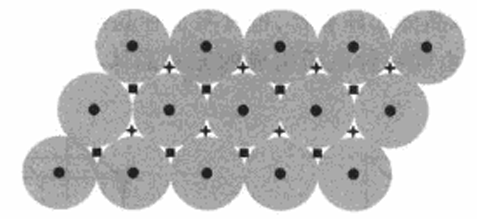
\includegraphics[height=4em, keepaspectratio=true]{pic/1-06} & 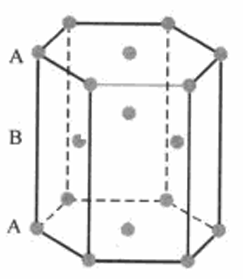
\includegraphics[height=8em, keepaspectratio=true]{pic/1-07} & 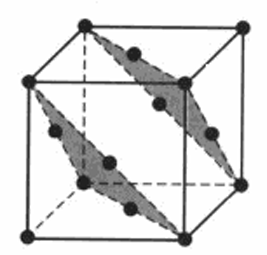
\includegraphics[height=8em, keepaspectratio=true]{pic/1-08}\\
            晶格常数$a$ & a & a \& c & a \\
            密排方向    &沿两近邻粒子方向$a=2r$&水平方向$a=2r$垂直方向$h=\frac{\sqrt{6}}{2}a=\frac{c}{2}$&沿面对角线$\sqrt{2}a=4r$\\
            有效原子数  &1&2&4\\
            配位数$n$   &6&12&12\\
            最近邻距离$a$&$a$&$a$&$\frac{\sqrt{2}}{2}a$\\
            致密度$\rho$&&$\rho_1=\frac{2\times \frac{4}{3} \pi r^3}{(\frac{\sqrt{3}}{4}a)^3 \times 2\times h} = \frac{\sqrt{2}}{6} \pi$&$\rho_2=\frac{4\times \frac{4}{3} \pi r^3}{(2\sqrt{2}r)^3} = \frac{\sqrt{2}}{6}\pi$\\
        \end{tabular}
        }
        \caption{密堆积结构晶格}
        \label{tab:1-3}
    \end{table}

    我们给出这样的两个要点:
    \begin{enumerate}[itemsep=0pt,parsep=0pt]
        \item \textbf{面心立方}既可以从立方体结构的角度考虑,而如果我们从立方体的体对角线看过去——这就是密堆积结构的ABC型。
        \item \textbf{面心立方}与\textbf{体心立方}互为倒格子。这将是\autoref{chap:2}的重要结论。
    \end{enumerate}

\subsubsection{第三类晶格:复式晶格}
    上述的第一类晶格与第二类晶格,常见于同一种原子所组成的单质晶体。我们现在介绍一些由多种原子或离子所组成的化合物晶体的晶格。

    我们介绍简单晶格与复式晶格的概念。化合物常表现为复式晶格。
    \begin{itemize}[itemsep=0pt,parsep=0pt]
        \item \textbf{简单晶格}\index{简单晶格}:所有原子完全等价。将晶格从一个原子向另一个原子作平移后,新得到的晶格与原晶格完全复原。
        \item \textbf{复式晶格}\index{复式晶格}:含有两种及以上不等价的所有原子或离子。将晶格从一个粒子向另一个粒子作平移后,无法复原晶格。复式晶格总可以看成若干种简单晶格的套构。
    \end{itemize}

    我们以下面三种化合物晶体为例,研究复式晶格及其套构。

    \textbf{CsCl结构}\index{CsCl结构}:CsCl结构与体心立方类似,但位于体心与位于顶点的分别是两种不同的离子,每种离子位于8个异类离子构成的立方体的中心。如果考虑整个晶格,“顶点”与“体心”的概念是相对的,二者完全等效。

    \textbf{NaCl结构}\index{NaCl结构}:将$Na^+$离子和$Cl^-$离子交替放在一个简单立方晶格上,构成NaCl结构。显然$Na^+$离子与$Cl^-$离子两类粒子不等价。实际上所有的碱金属-卤化物晶体都具有NaCl结构。

    \textbf{ZnS结构}\index{金刚石结构}:闪锌矿ZnS的结构与面心立方类似,由面心立方的中心到各个顶角作8条对角线,并在其中4条互不相邻的对角线的中点放置另一种粒子。两种粒子位置不等价,每种粒子处于4个最近邻异类粒子所构成的四面体的中心。两种粒子各自构成的四面体在取向上相差$90^{\circ}$。金刚石与半导体材料锗、硅也具有该结构。

    归纳复式晶格如\autoref{tab:1-4}所示:
    \begin{table}[!htbp]
        \centering
        \resizebox{\textwidth}{!}{
        \setlength{\tabcolsep}{1em}
        \begin{tabular}{cccc}
                & CsCl结构 & NaCl结构 & 金刚石结构\\
                & 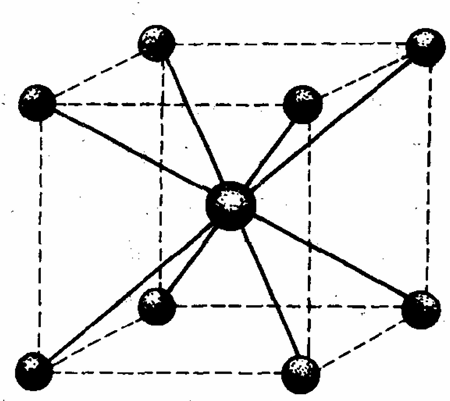
\includegraphics[height=8em, keepaspectratio=true]{pic/1-12} & 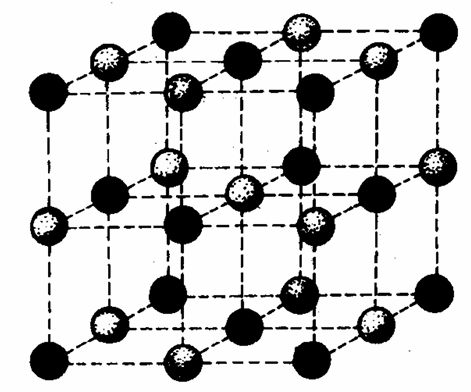
\includegraphics[height=8em, keepaspectratio=true]{pic/1-13} & 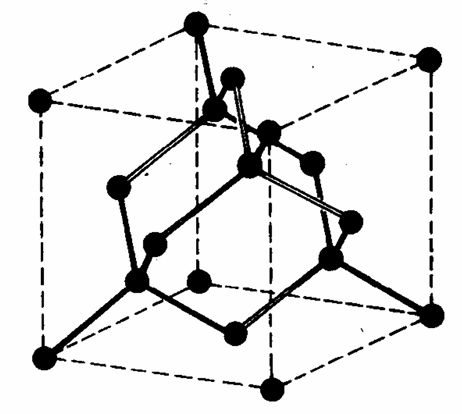
\includegraphics[height=8em, keepaspectratio=true]{pic/1-14}\\
            有效原子数  &2&8&8\\
            配位数$n$   &8&6&4\\
            套构情况    &简单立方沿对角线方向$\frac{1}{2}$套构&面心立方沿棱方向$\frac{1}{2}$套构&体心立方沿对角线方向$\frac{1}{4}$套构\\
        \end{tabular}
        }
        \caption{复式晶格}
        \label{tab:1-4}
    \end{table}
    
\section{晶体的周期性}\index{晶体的周期性}\label{sec:1-2}
    凡是晶体就具有\textbf{周期性},也称为平移对称性。我们可以用一个最小的、完全等价的结构单元,在空间无限重复,从而得到整个晶格。这个能够充分反映晶体结构特征的全同结构单元称为\textbf{晶胞}\index{晶胞}或\textbf{基元}。晶胞有多种选取方式,最实用的是单胞与原胞两种。

    为了研究晶体的周期性即平移对称性,我们忽略晶体中的具体粒子,将不等价的粒子(即基元)抽象为几何点,从而原本复杂的晶格被抽象为纯粹的几何点阵。这样的点阵称为\textbf{布拉菲点阵}或\textbf{布拉菲格子}\index{布拉菲格子}。

\subsection{布拉菲点阵}
    布拉菲点阵作为数学概念,是由分立点所构成的无限阵列,从阵列的任何一个结点去看,周围各结点的分布与方位都是精确相同的。

    对于晶格来说,我们通过将基元抽象为几何点得到布拉菲格子。于是我们有:
    \[
        \mbox{<晶体>}=\mbox{<基元>}+\mbox{<布拉菲点阵>}
    \]
    
    我们考虑二维平面与三维空间中有多少种布拉菲格子,即几何点在二维平面(三维空间)有多少种周期性的规律排布。

\subsubsection{二维布拉菲格子}
    共存在5种二维布拉菲格子,又可分为4种晶系。我们记二维点阵的两边为$a$、$b$,第三边为$c$;夹角为$\gamma$,其分类标准及转化关系如\autoref{tab:1-5}所示:

    \begin{table}[!htbp]
        \centering
        \resizebox{\textwidth}{!}{
        \setlength{\tabcolsep}{1em}
        \begin{tabular}{ccccc}
            \toprule
            布拉菲格子& 边长特征        & 夹角特征                   & 晶系     & 转化关系 \\
            \midrule
            斜方      & $a\neq b$      & $\gamma \neq 90^{\circ}$  & 斜方晶系 & \multirow{5}{*}[-0.5em]{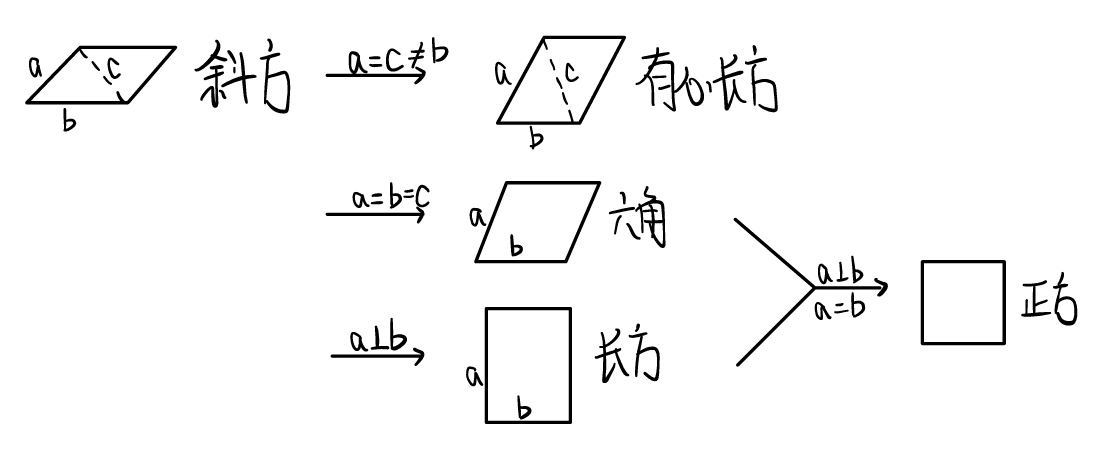
\includegraphics[height=7em, keepaspectratio=true]{pic/1-16}}\\
            有心长方  & $a = c \neq b$ & $\gamma \neq 90^{\circ}$  & \multirow{2}{*}{长方晶系} &\\
            长方      & $a\neq b$      & $\gamma=90^{\circ}$       &         &  \\
            六角      & $a=b$          & $\gamma=60^{\circ}$       & 六角晶系 &  \\
            正方      & $a=b$          & $\gamma=90^{\circ}$       & 正方晶系 &  \\
            \bottomrule
        \end{tabular}
        }
        \caption{二维布拉菲格子}
        \label{tab:1-5}
    \end{table}

    \autoref{fig:1-05}可以证明,左侧的所谓“有心正方”晶格实际上等价于“正方”,即5种二维布拉菲格子已经完备。

    \begin{figure}[!htbp]
        \centering
        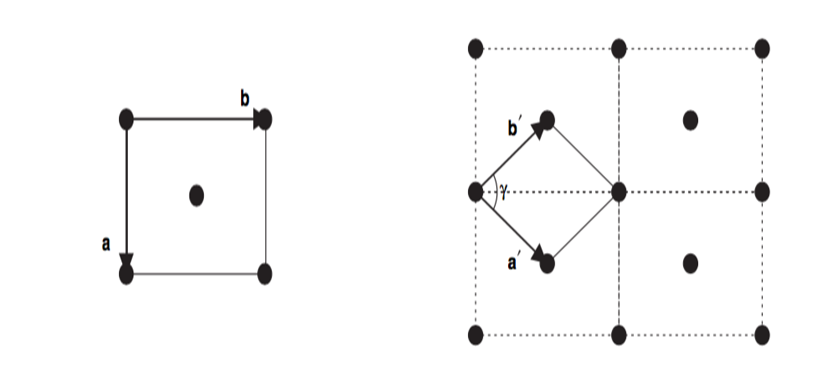
\includegraphics[height=9em, keepaspectratio=true]{pic/1-17}
        \caption{不存在“有心正方”晶格}
        \label{fig:1-05}
    \end{figure}

\subsubsection{三维布拉菲格子}
    共存在14种二维布拉菲格子,又可分为7种晶系。我们记三维点阵的三边为$a$、$b$、$c$,三个方向的夹角为$\alpha$、$\beta$、$\gamma$。如\autoref{tab:1-6}所示:

    \begin{table}[!htbp]
        \centering
        \resizebox{\textwidth}{!}{
        \setlength{\tabcolsep}{1em}
        \begin{tabular}{ccccc}
            \toprule
            晶系     & 边长特征         & 夹角特征                   & 布拉菲格子  & 示意图 \\
            \midrule
            三斜晶系 & $a\neq b\neq c$ & $\alpha \neq \beta \neq \gamma$                 & 简单三斜    & \multirow{7}{*}[-1.5em]{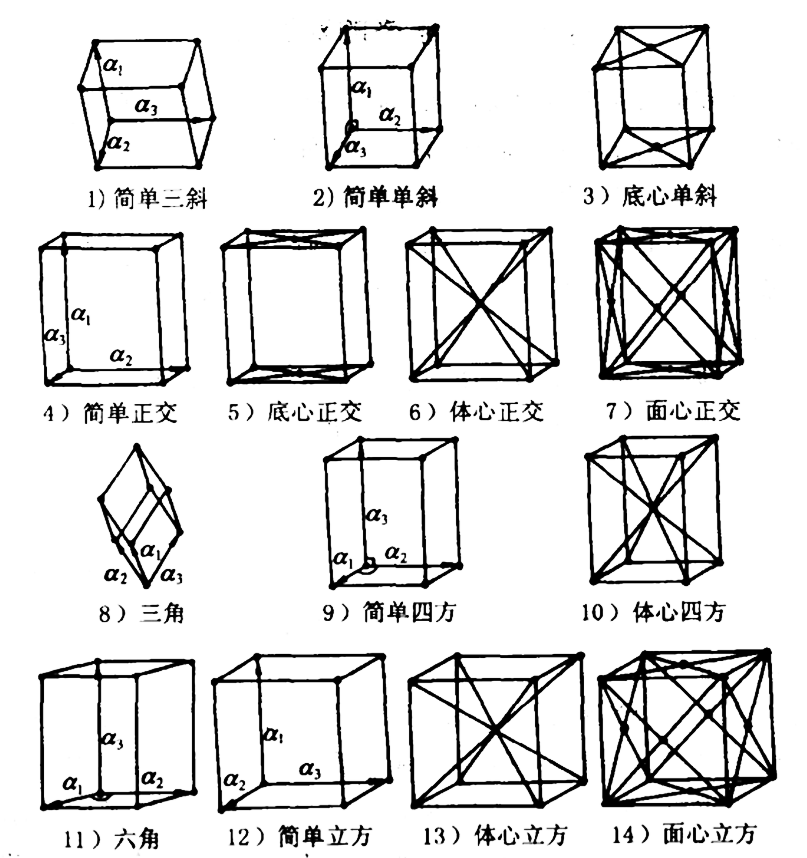
\includegraphics[height=10em, keepaspectratio=true]{pic/1-18}} \\
            单斜晶系 & $a\neq b\neq c$ & $\alpha=\gamma=90^{\circ}\neq \beta $           & 简单单斜、底心单斜    & \\
            三角晶系 & $a=b=c$         & $\alpha=\beta=\gamma\neq90^{\circ}<120^{\circ}$ & 三角    & \\
            正交晶系 & $a\neq b\neq c$ & $\alpha=\beta=\gamma=90^{\circ}$                & \makecell{简单正交、底心正交、\\体心正交、面心正交}    & \\
            四角晶系 & $a=b\neq c$     & $\alpha=\beta=\gamma=90^{\circ}$                & 简单四角、体心四角    & \\
            六角晶系 & $a=b\neq c$     & $\alpha=\beta=90^{\circ}, \gamma=120^{\circ}$   & 六角    & \\
            正方晶系 & $a=b=c$         & $\alpha=\beta=\gamma=90^{\circ}$                & \makecell{简单立方、体心立方、\\面心立方}    & \\
            \bottomrule
        \end{tabular}
        }
        \caption{三维布拉菲格子}
        \label{tab:1-6}
    \end{table}

    与二维平面不存在所谓“有心正方”同理,三维空间不存在所谓“底心立方”、“面心正方”、“体心单斜”晶格,实际上等价于“简单立方”、“体心正方”、“底心单斜”,证明如\autoref{fig:1-06}所示。这也说明了14种三维布拉菲格子的完备性。

    \begin{figure}[!htbp]
        \centering
        \begin{minipage}[t]{0.3\linewidth}
            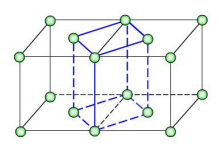
\includegraphics[width=1\linewidth, keepaspectratio=true]{pic/1-19}
            \subcaption{“底心立方”}
        \end{minipage}
        \hfill
        \begin{minipage}[t]{0.3\linewidth}
            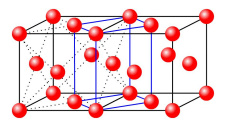
\includegraphics[width=1\linewidth, keepaspectratio=true]{pic/1-20}
            \subcaption{“面心正方”}
        \end{minipage}
        \hfill
        \begin{minipage}[t]{0.3\linewidth}
            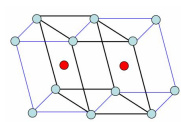
\includegraphics[width=1\linewidth, keepaspectratio=true]{pic/1-21}
            \subcaption{“体心单斜”}
        \end{minipage}
        \caption{不存在“底心立方”、“面心正方”、“体心单斜”晶格}
        \label{fig:1-06}
    \end{figure}

    布拉菲点阵是晶格的数学抽象。只要将基元按照布拉菲点阵排布,就可以还原晶体结构。同一种布拉菲点阵可以对应不同的晶体结构,但其平移对称性是一致的。

\subsection{单胞和原胞}
    三维晶格的晶胞通常是一个平行六面体,沿着某点出发的三条边取单位矢量$\vec{a_1}$、$\vec{a_2}$、$\vec{a_3}$,即晶胞的单位边矢量,这就是\textbf{晶格基矢}\index{晶格基矢}。晶胞所占的体积$\Omega=(\vec{a_1}\cdot \vec{a_2})\times \vec{a_3}$。

    现在研究晶胞的选取,常选取单胞或原胞作为晶胞:
    \begin{itemize}[itemsep=0pt,parsep=0pt]
        \item \textbf{单胞}\index{单胞}:反映晶格的宏观对称特性,常选取立方晶胞,其三条基矢沿着晶体的结晶轴方向,且尽可能构成正交系。
        \item \textbf{原胞}\index{原胞}:指晶格体积最小的周期性单元,可通过任意两结点的平移矢量$\vec{R}$不重不漏密排整个空间。原胞中只含有一个结点。原胞的三条基矢沿原胞的边的方向。
    \end{itemize}

    实际上单胞与原胞有多种取法。在晶体学中对各种晶格的单胞与原胞的选取做了规定,\autoref{tab:1-7}归纳了常用晶体所选取的单胞与原胞:
    \begin{table}[!htbp]
        \centering
        \resizebox{\textwidth}{!}{
        \setlength{\tabcolsep}{1em}
        \begin{tabular}{cclcl}
            \toprule
            晶格类型 & \multicolumn{2}{c}{单胞} & \multicolumn{2}{c}{原胞}\\
            \midrule
            简单立方 & 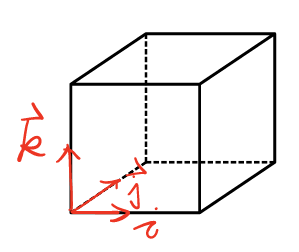
\includegraphics[valign=m, height=4em, keepaspectratio=true]{pic/1-22} & $
            \begin{cases}
            \vec{a_1}=a\vec{i}\\
            \vec{a_2}=a\vec{j}\\
            \vec{a_3}=a\vec{k}\\
            \end{cases}
            $ & 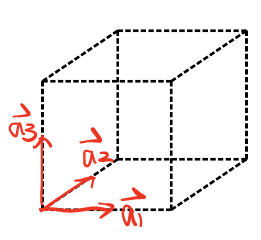
\includegraphics[valign=m, height=4em, keepaspectratio=true]{pic/1-24} & $
            \begin{cases}
            \vec{a_1}=a\vec{i}\\
            \vec{a_2}=a\vec{j}\\
            \vec{a_3}=a\vec{k}\\
            \end{cases}
            $ \\
            面心立方 & 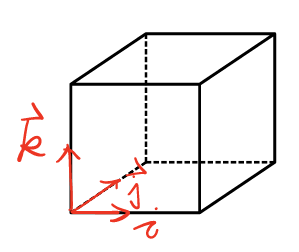
\includegraphics[valign=m, height=4em, keepaspectratio=true]{pic/1-22} & $
            \begin{cases}
            \vec{a_1}=a\vec{i}\\
            \vec{a_2}=a\vec{j}\\
            \vec{a_3}=a\vec{k}\\
            \end{cases}
            $ & 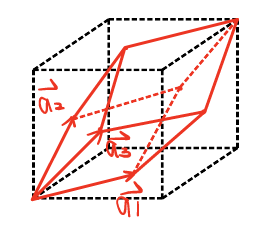
\includegraphics[valign=m, height=4em, keepaspectratio=true]{pic/1-25} & $
            \begin{cases}
            \vec{a_1}=\frac{a}{2}(\vec{i}+\vec{j})\\
            \vec{a_2}=\frac{a}{2}(\vec{j}+\vec{k})\\
            \vec{a_3}=\frac{a}{2}(\vec{k}+\vec{i})\\
            \end{cases}
            $ \\
            体心立方 & 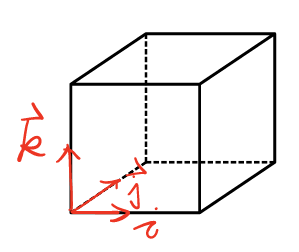
\includegraphics[valign=m, height=4em, keepaspectratio=true]{pic/1-22} & $
            \begin{cases}
            \vec{a_1}=a\vec{i}\\
            \vec{a_2}=a\vec{j}\\
            \vec{a_3}=a\vec{k}\\
            \end{cases}
            $ & 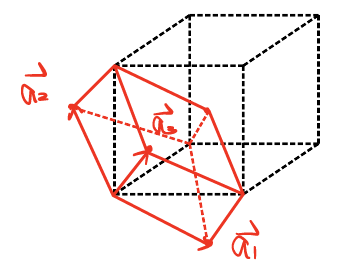
\includegraphics[valign=m, height=4em, keepaspectratio=true]{pic/1-26} & $
            \begin{cases}
            \vec{a_1}=\frac{a}{2}(\vec{i}+\vec{j}-\vec{k})\\
            \vec{a_2}=\frac{a}{2}(\vec{j}+\vec{k}-\vec{i})\\
            \vec{a_3}=\frac{a}{2}(\vec{k}+\vec{i}-\vec{j})\\
            \end{cases}
            $ \\
            六角密排 & 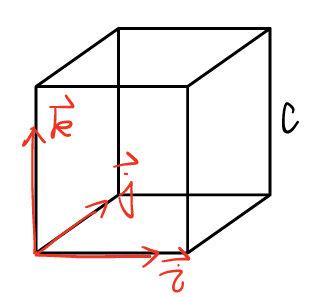
\includegraphics[valign=m, height=4em, keepaspectratio=true]{pic/1-23} & $
            \begin{cases}
            \vec{a_1}=a\vec{i}\\
            \vec{a_2}=a\vec{j}\\
            \vec{a_3}=c\vec{k}\\
            \end{cases}
            $ & 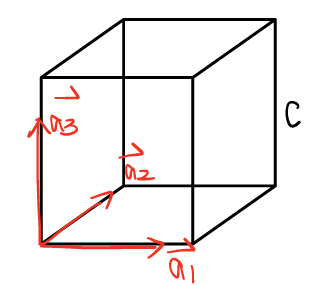
\includegraphics[valign=m, height=4em, keepaspectratio=true]{pic/1-27} & $
            \begin{cases}
            \vec{a_1}=a\vec{i}\\
            \vec{a_2}=\frac{a}{2}\vec{i}+\frac{\sqrt{3}a}{2}\vec{j}\\
            \vec{a_3}=c\vec{k}\\
            \end{cases}
            $ \\
            \bottomrule
        \end{tabular}
        }
        \caption{单胞与原胞的选取}
        \label{tab:1-7}
    \end{table}

    观察发现:单胞实际上是扩大了的原胞,是较大的周期单元;某些情况单胞与原胞相同。

\subsection{晶体的平移对称性}
\subsubsection{点阵的残缺的平移不变性}
    对于二维基矢$\{\vec{a_1}, \vec{a_2}\}$或三维基矢$\{\vec{a_1}, \vec{a_2}\, \vec{a_3}\}$,点阵中的自原点到每个结点的位置矢量$\vec{R_l}$可以写成
    \[
        \vec{R_l}=l_1\vec{a_1}+l_2\vec{a_2}+l_3\vec{a_3}
    \]
    其中$\{l_1, l_2, l_3\}$取任意整数时,位置矢量$\vec{R_l}$所指向的端点的集合将包含且仅包含整个点阵全部的结点。

    由此可知,点阵并不对任意的平移不变,而只对一组离散的平移矢量$\vec{R_l}$(其中$l_1, l_2, l_3\in \mathbb{N}$)具有不变性,称为残缺的平移不变性。

    此时,点阵中的任意结点由$l_1, l_2, l_3$的组合$(l_1, l_2, l_3)$唯一确定,布拉菲格子则是所有点$(l_1, l_2, l_3)$的集合。

\subsubsection{晶体物理性质的周期性}
    我们知道:
    \[
        \mbox{<晶体>}=\mbox{<基元>}+\mbox{<布拉菲点阵>}
    \]
    
    对于某个晶胞基元,其中第$\alpha$个粒子相对于晶胞原点有相对位移$\vec{r_\alpha}$。实际的晶格可以看成:在布拉菲点阵的每个结点上放置一个晶胞基元,晶胞基元中的粒子与结点间的相对位移即为$\vec{r_\alpha}$。只要将晶胞基元按照布拉菲格子排布,就能得到晶体的结构。

    则此时晶格中任意粒子的位置矢量可以写为:
    \[
        \vec{R_l}=\vec{r_\alpha}+l_1\vec{a_1}+l_2\vec{a_2}+l_3\vec{a_3}
        \quad (\alpha = 1,2,\dots)
    \]

    如果晶体中所有晶胞基元都严格处在布拉菲格子所确定的结点上,那么晶体内的一切物理量$V(\vec{r})$,都精确的是$\vec{R_l}$的周期函数,即:
    \[
        V(\vec{r})=V(\vec{r}+\vec{R_l})
    \]
    其中$\vec{r}$是坐标原点到任意位置的位移矢量。\label{tag:Crystal_Periodicity}

\section{晶体的方向性}\index{晶体的方向性}
    晶体的一个基本特点是具有\textbf{方向性},沿晶格的不同方向晶体性质不同。这种性质差异被称为\textbf{各向异性}\index{各向异性}。这是因为单晶材料内部原子排列具有方向性,不同晶面方向上,原子的排列密度、原子间的结合强度、电子的运动方式等等都会有所不同,从而导致性质上的差异。

    我们在本节关注如何区别和描述晶格中的方向。
\subsection{晶向}
\subsubsection{晶列}
    在布拉菲点阵中,过原点和任意的一个结点可以确定一条直线。由于结点呈周期性排列,用一族这样平行且等间距的直线可以将整个点阵包括无遗,如\autoref{fig:1-07}中的虚线或实线所示。这样的一族直线我们称为\textbf{晶列}\index{晶列}。

    \begin{figure}[!htbp]
        \centering
        \begin{minipage}[t]{0.45\linewidth}
            \centering    
            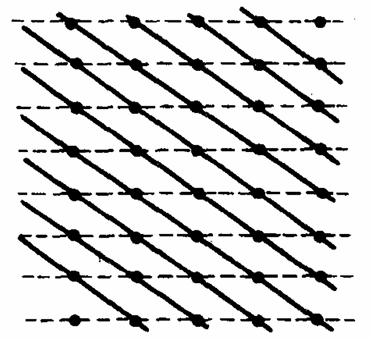
\includegraphics[height=8em, keepaspectratio=true]{pic/1-28}
            \caption{晶列}
            \label{fig:1-07}
        \end{minipage}
        \hfill
        \begin{minipage}[t]{0.45\linewidth}
            \centering
            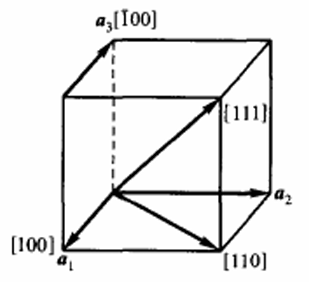
\includegraphics[height=8em, keepaspectratio=true]{pic/1-29}
            \caption{简单立方晶格的晶向}
            \label{fig:1-08}
        \end{minipage}
    \end{figure}
    
    由于布拉菲点阵中有无限个结点,也就有无限多条方向彼此不同的直线族,从而点阵中有无限族晶列。每一族晶列确定了一个方向,即\textbf{晶向}\index{晶向}。如果从一个结点沿着某晶列方向到最近邻结点的平移矢量为:
    \[
        \vec{R_l}=l_1\vec{a_1}+l_2\vec{a_2}+l_3\vec{a_3}
    \]
    则用$l_1$、$l_2$、$l_3$标志该晶列所对应的晶向,记为$[l_1, l_2, l_3]$,称为\textbf{晶向指数}\index{晶向指数}。由于平移矢量$\vec{R_l}$是最近邻原子间的位移,$l_1$、$l_2$、$l_3$一定是互质的整数,按照惯例若$l_1$、$l_2$、$l_3$为负数,则上标一横,如$-l_i$记为$\overline{l_i}$。

    以简单立方晶格中的晶向为例,如\autoref{fig:1-08}所示,其边、面对角线、体对角线的晶向指数依次为$[100]$、$[110]$、$[111]$。

\subsubsection{等效晶向}
    由于晶格具有对称性,某些晶向上晶格结构和晶学性质是相同的,我们称这些晶向是等效的,即\textbf{等效晶向}\index{等效晶向}。

    例如,立方晶格的边一共有$[100]$、$[\overline{1}00]$、$[010]$、$[0\overline{1}0]$、$[001]$、$[00\overline{1}]$六个晶向,考虑晶格的平移对称性,晶体在这些方向上的性质是完全相同的。我们用$<l_1,l_2,l_3>$来标志一组对称且等效的晶向,即$<100>$。

    边晶向、面对角线晶向、体对角线晶向总结如\autoref{tab:1-8}所示:
    \begin{table}[!htbp]
        \centering
        \resizebox{\textwidth}{!}{
        \setlength{\tabcolsep}{1em}
        \begin{tabular}{cccc}
                   & 边       & 面对角线 & 体对角线  \\
                   & 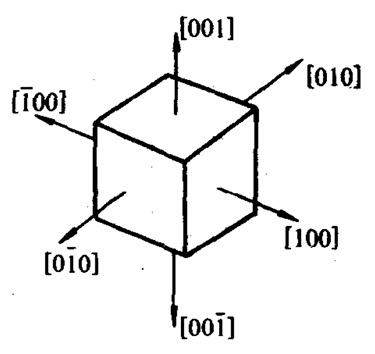
\includegraphics[height=8em, keepaspectratio=true]{pic/1-30} & 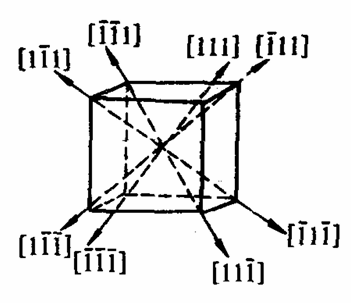
\includegraphics[height=8em, keepaspectratio=true]{pic/1-31} & 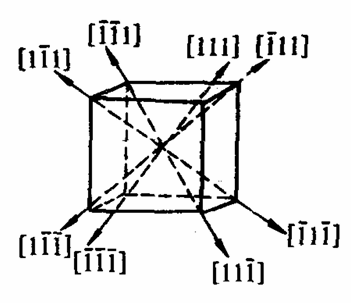
\includegraphics[height=8em, keepaspectratio=true]{pic/1-32} \\
            数目    & 6       &     12  &     8    \\
            等效晶向& $<100>$ & $<110>$ & $<111>$ \\
        \end{tabular}
        }
        \caption{等效晶向}
        \label{tab:1-8}
    \end{table}

    \textcolor{red}{一般晶向用$[l_1, l_2, l_3]$标志,系列晶向用$<l_1,l_2,l_3>$标志}

\subsection{晶面}
\subsubsection{晶面}
    在布拉菲点阵中,由于结点呈周期性排列,用一族平行且等间距的平面可以将整个点阵包括无遗,如\autoref{fig:1-09}所示。这样的一族平面我们称为\textbf{晶面}\index{晶面}。

    \begin{figure}[!htbp]
        \centering    
        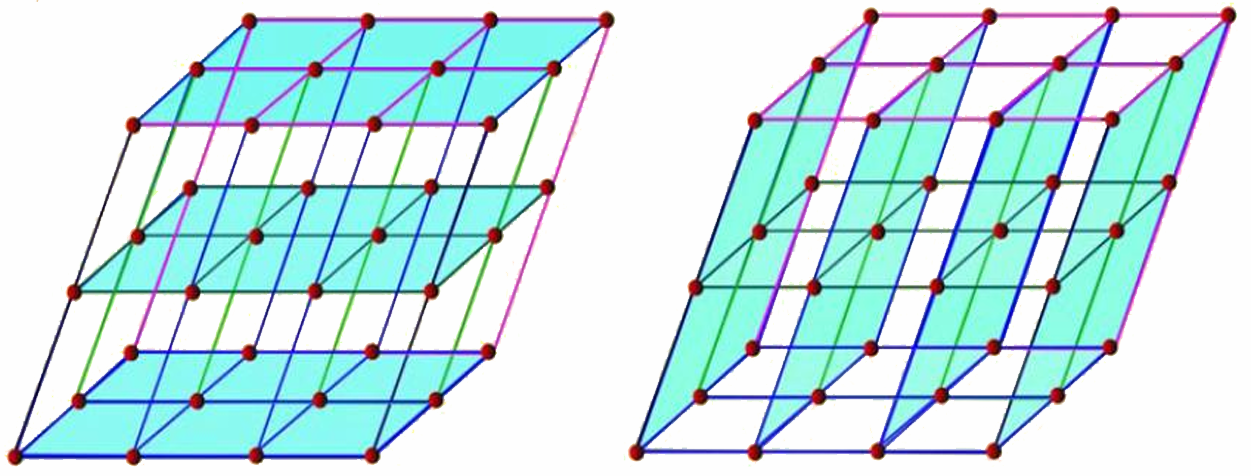
\includegraphics[height=7em, keepaspectratio=true]{pic/1-33}
        \caption{晶面}
        \label{fig:1-09}
    \end{figure}

    由于布拉菲点阵中有无限个结点,也就有无限多个方向彼此不同的平面族,从而点阵中有无限族晶面。每一族晶面确定了一个方向,即该族平面的法线方向。在数学上,我们可以用该平面法线的方向余弦,或者该平面在坐标轴上的截距来描述一个平面的方向——我们接下来将看到,这两种表示实际上是等价的。

    对于晶格中的一组平行且等距的晶面,将完全无遗地包括所有结点选取某个结点作为原点,以晶胞基矢为坐标轴建立坐标系,如\autoref{fig:1-10}所示。
    
    记晶面的法线方向为$\vec{e_n}$,晶面间距为$d$。指向第$\mu$个晶面($\mu$为整数)任意位置的位矢为$\vec{X}$,该晶面在坐标轴上的截距依次为$r_\mu a$、$s_\mu a$、$t_\mu a$。

    \begin{figure}[!htbp]
        \centering    
        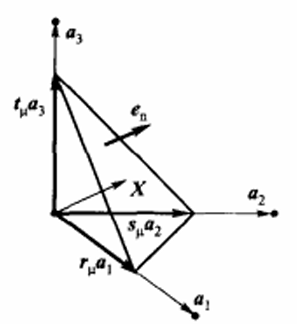
\includegraphics[height=8em, keepaspectratio=true]{pic/1-34}
        \caption{晶面的方向余弦}
        \label{fig:1-10}
    \end{figure}

    则有
    \[
        \vec{X} \cdot \vec{e_n} = \mu d
    \]
    
    将该晶面与坐标轴的交点代入可得:
    \[
    \begin{cases}
        r_\mu \vec{a_1} \cdot \vec{e_n} = r_\mu \cos (\vec{a_1}, \vec{e_n}) = \mu d \\
        s_\mu \vec{a_2} \cdot \vec{e_n} = s_\mu \cos (\vec{a_2}, \vec{e_n}) = \mu d \\
        t_\mu \vec{a_1} \cdot \vec{e_n} = t_\mu \cos (\vec{a_3}, \vec{e_n}) = \mu d \\
    \end{cases}
    \]

    联立可得:
    \[
        \cos (\vec{a_1}, \vec{e_n}) : \cos (\vec{a_1}, \vec{e_n}) : \cos (\vec{a_1}, \vec{e_n}) = \frac{1}{r_\mu} : \frac{1}{r_\mu} : \frac{1}{r_\mu}
    \]

    即:晶面法线方向的方向余弦之比,等于晶面与对应方向坐标轴截距的倒数之比。因此方向余弦和截距表述晶面方向是等价的,常用晶面与坐标轴的截距来表示晶面方向。

    进一步证明该组截距均为有理数。考察单位基矢处的结点,即$(1,0,0)$、$(0,1,0)$、$(0,0,1)$三个结点,由于晶面完全无遗包括所有结点,必然存在若干晶面经过该三个结点。不失一般的,我们记第$\mu_1$、$\mu_2$、$\mu_3$个晶面经过这三个结点。某些情况下可能存在一个晶面同时经过多个结点,此时相应地调整$\mu_1=\mu_2$即可。

    于是,第$\mu_i$个晶面在$\vec{a_i}$坐标轴上的截距为单位1,从而第$\mu$个晶面在坐标轴上的截距有:
    \[
        r_\mu = \frac{\mu}{\mu_1}, \\
        s_\mu = \frac{\mu}{\mu_2}, \\
        t_\mu = \frac{\mu}{\mu_3}
    \]
    其中$\mu$、$\mu_1$、$\mu_2$、$\mu_3$均为整数。
    
    则$r_\mu a$、$s_\mu a$、$t_\mu a$均是两个整数之比,必为有理数。

\subsubsection{晶面指数}
    若第一个晶面在坐标轴上的截距为$r_1 a$、$s_1 a$、$t_1 a$,取截距的倒数$h_1 = \frac{1}{r_1 a}, h_2 = \frac{1}{s_1 a}, h_3 = \frac{1}{t_1 a}$来标志该族晶面。若晶面在坐标轴上无截距,即截距无穷大,规定倒数为0。定义$(h_1, h_2, h_3)$为晶面指数,用来反映晶面所确定的方向。一般要求$h_1, h_2, h_3$互质。

    确定晶面指数的程序可以归纳为:
    \begin{enumerate}[itemsep=0pt,parsep=0pt]
        \item \textbf{找截距}:找出任一晶面在基矢坐标轴上的截距$r$、$s$、$t$;
        \item \textbf{取倒数}:取截距的倒数$h_1 = \frac{1}{r}, h_2 = \frac{1}{s}, h_3 = \frac{1}{t}$;
        \item \textbf{化互质}:确保晶面指数$(h_1, h_2, h_3)$互质。负数则在上方画一横线表示。
    \end{enumerate}

    立方结构晶格主要晶面如\autoref{fig:1-11}所示。

    \begin{figure}[!htbp]
        \centering    
        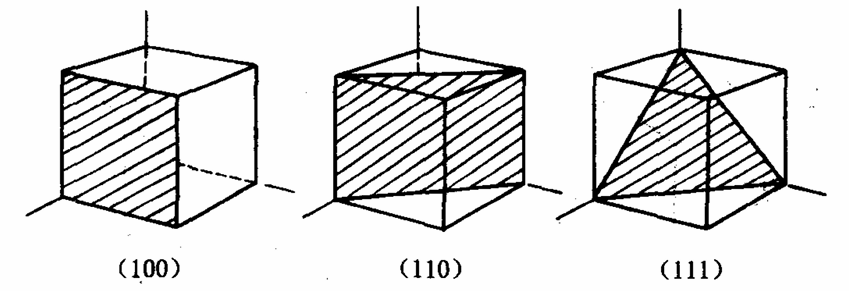
\includegraphics[height=8em, keepaspectratio=true]{pic/1-35}
        \caption{晶面指数}
        \label{fig:1-11}
    \end{figure}

    与等效晶向同理,我们认为具有相同晶体性质的晶面是等效的,即\textbf{等效晶面}\index{等效晶面}。

    例如,立方晶格的表面一共有$(100)$、$(\overline{1}00)$、$(010)$、$(0\overline{1}0)$、$(001)$、$(00\overline{1})$六个晶面,考虑晶格的平移对称性,晶体在这些晶面上的性质是完全相同的。我们用$\{h_1,h_2,h_3\}$来标志一组对称且等效的晶面,即$\{100\}$。

    等效晶面总结如\autoref{tab:1-9}所示:
    \begin{table}[!htbp]
        \centering
        \resizebox{\textwidth}{!}{
        \setlength{\tabcolsep}{1em}
        \begin{tabular}{ccccc}
            \toprule
            &   晶面     & 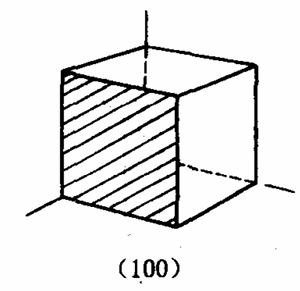
\includegraphics[valign=m, height=4em, keepaspectratio=true]{pic/1-36} & 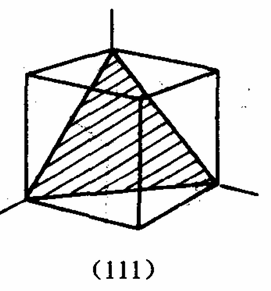
\includegraphics[valign=m, height=4em, keepaspectratio=true]{pic/1-37} & 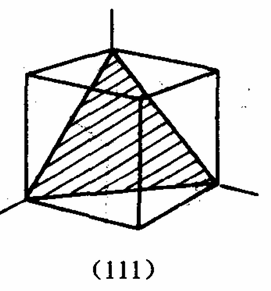
\includegraphics[valign=m, height=4em, keepaspectratio=true]{pic/1-38} \\ \\
            \hline
            \multirow{3}{*}{\textbf{晶向}} & 法线     & 边 & 面对角线 & 体对角线  \\
                                           & 法线数   & 6 & 12 & 8 \\
                                           & 等效晶向 & $<100>$ & $<110>$ & $<111>$ \\
            \hline
            \multirow{3}{*}[-3em]{\textbf{晶面}} & 晶面数   & 6 & 12 & 8 \\
                                           & 等效晶面 & 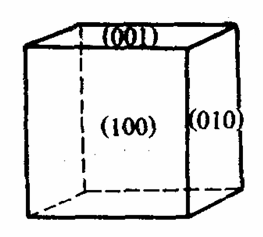
\includegraphics[valign=m, height=3em, keepaspectratio=true]{pic/1-39} & 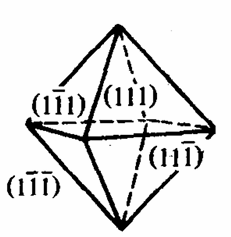
\includegraphics[valign=m, height=3em, keepaspectratio=true]{pic/1-40} & 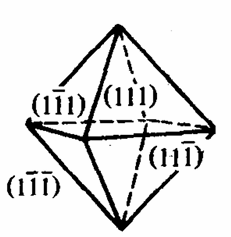
\includegraphics[valign=m, height=3em, keepaspectratio=true]{pic/1-41} \\
                                           & 等效晶面 & $\{100\}$ & $\{110\}$ & $\{111\}$ \\
            \bottomrule
        \end{tabular}
        }
        \caption{等效晶面}
        \label{tab:1-9}
    \end{table}

\subsubsection{密勒指数}
    无论是晶向指数还是晶面指数,都依托于所选取的基矢。
    
    当所选取的晶胞是单胞时,记此时的晶面指数为\textbf{密勒指数}\index{密勒指数},用$\{h, k, l\}$表示;当所选取的晶胞是原胞时,记此时的晶面指数为$\{h_1, h_2, h_3\}$。

    如\nameref{tab:1-7}所述,考虑到:
    \begin{itemize}[itemsep=0pt,parsep=0pt]
        \item 单胞与原胞的基矢在方向、长度上可能不同;
        \item 单胞实际上是扩大了的原胞,从而原胞可以完全反映布拉菲格子的平移对称性,而单胞所反映的对称性是基于平移矢量$\vec{R_l}$的子集,只能沿着结晶轴方向,从而只能局部反映布拉菲格子的平移对称性。
    \end{itemize}
    通过沿坐标轴方向平移单胞,可能无法得到所有的布拉菲格子中的结点,存在遗漏的可能性,进而导致晶面指数中某些晶面的丢失。

    如\autoref{fig:1-12}所示,左侧采用原胞,右侧采用单胞。从而左侧完全无遗地包含所有结点,而右侧的单胞做平移,将沿结晶轴方向平移晶格常数$a$,将无法包含黄色晶面所示的若干结点。右图中黄色晶面,若采用左图的原胞基矢,计算晶面指数为$(101)$,而采用右图的单胞基矢,计算密勒指数为$(100)$,即存在晶面的丢失,这也正是单胞平移时遗漏的结点所构成的晶面。

    \begin{figure}[!htbp]
        \centering    
        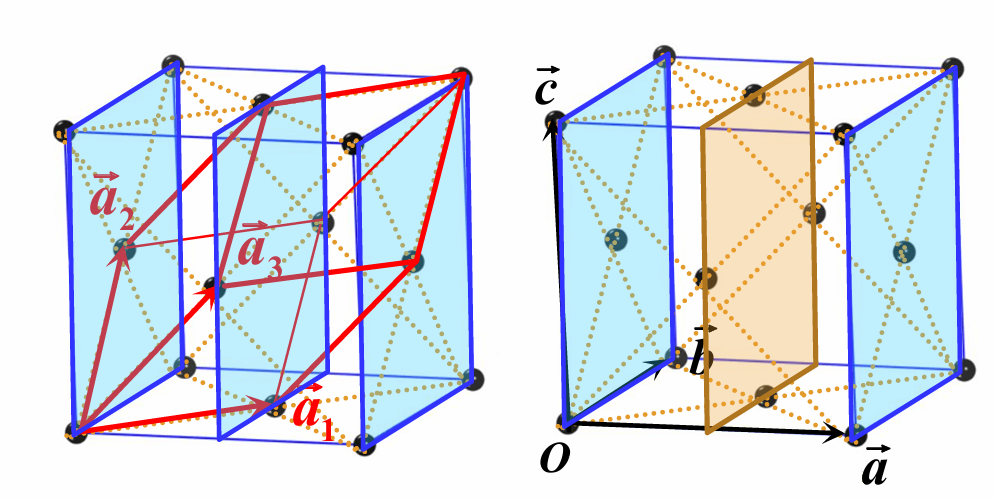
\includegraphics[height=11em, keepaspectratio=true]{pic/1-42}
        \caption{单胞可能导致晶面的丢失}
        \label{fig:1-12}
    \end{figure}

    因此立方单胞的密勒指数可能与其原胞的晶面指数不同。可以证明,立方体结构中,晶面的密勒指数与晶面法线方向的晶向指数完全相同。当密勒指数与晶面指数一致时,可以通过计算晶向指数,快速得到晶面指数,这也是计算晶面指数的另一种方法。
    
    具体来说,\autoref{tab:1-9}中就给出了立方体结构晶格常用晶面的晶面指数,及其法线的晶向指数——二者是完全相同的。

\section{晶体的宏观对称性}
    我们在\nameref{sec:1-2}一节,研究了晶体的周期性,即晶体的平移对称性,这也是固体理论中最重要的性质。具体来说,晶体通过平移矢量$\vec{R_l}$进行平移后,晶格可以完全复位。
    
    而实际上,晶体还具有另一类对称性:\textbf{点对称性},也称为\textbf{宏观对称性}。晶体中的粒子是周期性规律排列的,布拉菲格子是所有晶体的共同性质,基于粒子的周期排列,产生了不同晶体所具备的、不同的宏观对称性。

    所谓\textbf{宏观对称性}\index{宏观对称性},即晶体绕着某条轴进行旋转、绕着某个点进行反演操作后,晶格可以完全复位的性质。由于旋转或反演过程中,晶体至少有一个结点保持不动,整个晶体未进行平移操作,所以我们也称为\textbf{点对称性}\index{点对称性}。
    
\subsection{旋转与反演}
\subsubsection{变换矩阵}
    从数学的角度考虑对晶体做几何变换,即:
    \[
    \left(
    \begin{array}{c}
        x \\
        y \\
        z \\
    \end{array}
    \right)
    \stackrel{D}{\longrightarrow}
    \left(
    \begin{array}{c}
        x' \\
        y' \\
        z' \\
    \end{array}
    \right)
    =
    D
    \left(
    \begin{array}{c}
        x \\
        y \\
        z \\
    \end{array}
    \right)
    =
    \left(
    \begin{array}{ccc}
        d_{11} & d_{12} & d_{13} \\
        d_{21} & d_{22} & d_{23} \\
        d_{31} & d_{32} & d_{33} \\
    \end{array}
    \right)
    \left(
    \begin{array}{c}
        x \\
        y \\
        z \\
    \end{array}
    \right)
    \]
    其中$D$为变换矩阵,反映对晶体所做的几何变换:
    \[
    D=
    \left(
    \begin{array}{ccc}
        d_{11} & d_{12} & d_{13} \\
        d_{21} & d_{22} & d_{23} \\
        d_{31} & d_{32} & d_{33} \\
    \end{array}
    \right)
    \]
    
    我们考察变换矩阵$D$的性质。点对称操作是刚性操作,不会改变晶体的布拉菲格子,变换前后晶体中任意两点的距离不变:
    \begin{align*}
        x^2+y^2+z^2 & = x'^2+y'^2+z'^2\\
        (x,y,z)^T \cdot (x,y,z) & = (x',y',z')^T \cdot (x',y',z')\\
         & = (D\cdot(x,y,z))^T \cdot (D\cdot(x,y,z))\\
         & = (x,y,z)^T \cdot D^T \cdot D \cdot (x,y,z)\\
         & = (x,y,z)^T \cdot (D^T \cdot D) \cdot (x,y,z)
    \end{align*}

    因此要求变换矩阵$D$满足$D^T\cdot D = I$,其中$I$为单位矩阵。从而变换矩阵$D$是\textbf{正交矩阵},正交矩阵满足$D^{-1}=D^T$。

    考虑$D$的行列式的值。取行列式有$\left\lvert D\right\rvert^2=1$,从而变换矩阵$D$的行列式的值$\left\lvert D\right\rvert= \pm 1$。

\subsubsection{旋转操作、反演操作的变换矩阵}
    三维晶体的几何操作即正交变换,总可以表示成绕某一轴的旋转、对某中心的反演及其组合。
    
    因此我们可以将复杂的几何操作抽象为若干次基本的旋转、反演的叠加;矩阵上则是旋转矩阵和反演矩阵的相乘。

    因此我们给出旋转操作、反演操作的变换矩阵表示:
    \begin{itemize}[itemsep=0pt,parsep=0pt]
        \item 
        绕$z$轴旋转$\theta$的变换矩阵:
        \[
        D=
        \left(
        \begin{array}{ccc}
            \cos\theta & -\sin\theta & 0 \\
            \sin\theta & \cos\theta  & 0 \\
            0          & 0           & 1 \\
        \end{array}
        \right)
        ,\qquad\left\lvert D\right\rvert= 1
        \]
        其中$\theta$为旋转角。绕其他轴旋转同理。
        \item 
        绕原点做反演操作,也称中心反演的变换矩阵:
        \[
        D=
        \left(
        \begin{array}{ccc}
            -1 & 0 & 0 \\
            0 & -1 & 0 \\
            0 & 0 & -1 \\
        \end{array}
        \right)
        ,\qquad\left\lvert D\right\rvert= -1
        \]
    \end{itemize}
    应注意当变换矩阵表示旋转时的行列式的值取$1$;当变换矩阵表示反演时的行列式的值取$-1$。

\subsection{对称性、对称操作与对称素}
    从群论的角度,我们介绍对称性的概念如下:
    \begin{itemize}[itemsep=0pt,parsep=0pt]
        \item \textbf{对称性}\index{对称性}:经过对称操作后,系统保持不变的性质;
        \item \textbf{对称操作}\index{对称操作}:使得系统不变的操作;
        \item \textbf{对称素}\index{对称素}:对称操作所依赖的具体几何要素
    \end{itemize}

    对称操作可以概括系统的对称性。为了方便描述,有时不去列举具体的对称操作,而是描述系统所具有的对称素:
    \begin{itemize}[itemsep=0pt,parsep=0pt]
        \item 如果系统绕某轴旋转$\frac{2\pi}{n}$及其倍数不变,则称该轴为\textbf{$n$重旋转轴},记为$n$。
        \item 如果系统对某点反演不变,则称这个点为\textbf{对称心},记为$i$。
        \item 如果系统绕某轴旋转$\frac{2\pi}{n}$及其倍数后再反演不变,则称该轴为\textbf{$n$重旋转-反演轴},记为$\overline{n}$。
    \end{itemize}

\subsubsection{宏观对称性的破缺}
    如果是抽象的数学图形,它可能具有无穷多的对称操作及对称素。例如:球可以绕经过球心的任意轴线旋转任意角度,它有无数条无数重旋转(反演)轴;一条直线可以在上面的任何位置进行反演,其对称心有无数个。

    晶体则受制于具体晶格的限制。晶体本身经历对称操作不变,其布拉菲点阵经过对称操作也必须保持重合。晶体的宏观对称性是晶体中粒子规则排列的结果,也就必然受到平移对称性的制约:
    \begin{itemize}[itemsep=0pt,parsep=0pt]
        \item \textbf{对称操作及对称素有限}:只有绕着晶轴旋转某些特定角度,或关于某些特定结点进行反演,才有可能在操作后保持晶格不变。
        \item \textbf{对称素的组合有限}:对称素组合时受到严格限制,存在互斥关系与约束条件。
    \end{itemize}

\subsubsection{晶体的8种独立的对称素}
    基于这种破缺或限制,我们讨论对称操作及其对称素的可能取值。

    关注旋转操作。如\autoref{fig:1-13}所示,$A$、$B$是晶格中的两个结点,它们完全等价。关于$A$结点逆时针旋转$\theta$,原先的$B$结点来到$B'$位置;关于$B$结点顺时针旋转$\theta$,原先的$A$结点来到$A'$位置。为使晶体在旋转前后晶格不变,此处的$A'$、$B'$所在的位置在旋转前的晶格中必须存在结点。

    \begin{figure}[!htbp]
        \centering    
        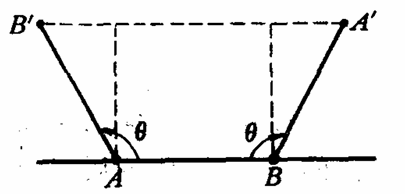
\includegraphics[height=8em, keepaspectratio=true]{pic/1-43}
        \caption{晶体的旋转操作}
        \label{fig:1-13}
    \end{figure}
    
    由几何关系可知$AB\mathop{//}A'B'$,从而
    \[
    \left\lvert A'B' \right\rvert = (1-2\cos \theta) \left\lvert AB\right\rvert= m\left\lvert AB\right\rvert
    \]
    其中$m$为整数,$\theta \in [0, 2\pi)$

    联立可得
    \begin{align*}
        m&=(1-2\cos \theta) \\
         &=-1,0,1,2,3  \\
        \theta&=0^\circ,60^\circ,90^\circ,120^\circ,180^\circ
    \end{align*}

    并依次对应$n=1,6,4,3,2$重旋转轴。

    考虑反演有$n=\overline{1},\overline{6},\overline{4},\overline{3},\overline{2}$重旋转-反演轴。

    综上,晶体中最多只存在十种对称素:
    \begin{table}[!htbp]
        \centering
        \resizebox{\textwidth}{!}{
        \setlength{\tabcolsep}{1em}
        \begin{tabular}{cccccc}
            \toprule
            旋转角度         & $360^\circ$ & $180^\circ$ & $120^\circ$ & $90^\circ$ & $60^\circ$ \\
            \midrule
            $n$重旋转轴      & 1 & 2 & 3 & 4 & 6 \\
            $n$重旋转-反演轴 & $\overline{1}$ & $\overline{2}$ & \textcolor{blue}{$\overline{3}$} & $\overline{4}$ & \textcolor{blue}{$\overline{6}$} \\
            \bottomrule
        \end{tabular}
        }
        \caption{晶体中的十种对称素}
        \label{tab:1-10}
    \end{table}

    应注意十种对称素中,$\overline{3}$等价于$3+\overline{1}$,$\overline{6}$等价于$\overline{3}+\overline{2}$,即它们可以由其他对称素导出。因此晶体中独立的对称素共$1,2,3,4,6,\overline{1},\overline{2},\overline{4}$共8种。

    对称素组合时,对称轴间的夹角、对称轴的数目等受到严格限制。举例来说:若晶体具有两条2重轴,其夹角必定为$30^{\circ}$、$45^{\circ}$、$60^{\circ}$、$90^{\circ}$中的一个;晶体最多就有一条6重轴;晶体的6重轴与4重轴不可能相交$\dots$

\subsection{宏观对称性与点群}
    晶体的\textbf{宏观对称性}\index{宏观对称性}要求考察该晶体的所有对称操作:对称操作越多,其宏观对称性越高。将晶体中全部对称操作的集合称为\textbf{对称操作群}\index{对称操作群}。基于\autoref{tab:1-10}所述的十种对称素所构成的对称操作群称为\textbf{点群}\index{点群}。
    
    从而晶体的宏观对称性可以用点群描述,宏观对称性不同的晶体属于不同的点群。

\subsubsection{立方点群$O_h$的对称性}
    我们考虑立方点群$O_h$的对称性。我们先讨论关于对称点的不动与反演操作,随后关注不同轴线作为对称素时的旋转(反演)操作——此时不考虑不动与反演即可:
    \begin{itemize}[itemsep=0pt,parsep=0pt]
        \item \textbf{不动与反演}:立方点群包括不动操作与反演操作。
        \item \textbf{对于三条立方轴}:每根轴线作为4重旋转轴及4重旋转反演轴,包括绕立方轴旋转$90^{\circ}$、$180^{\circ}$、$270^{\circ}$;绕立方轴旋转$90^{\circ}$、$180^{\circ}$、$270^{\circ}$再反演的六个对称操作。三条立方轴共计18个对称操作。
        \item \textbf{对于六条面对角线轴}:每根轴线作为2重旋转轴及2重旋转反演轴,包括绕面对角线轴旋转$180^{\circ}$;绕面对角线轴旋转$180^{\circ}$再反演的两个对称操作。六条面对角线轴共计12个对称操作。
        \item \textbf{对于四条体对角线轴}:每根轴线作为3重旋转轴及3重旋转反演轴,包括绕体对角线轴旋转$120^{\circ}$、$240^{\circ}$;绕体对角线轴旋转$120^{\circ}$、$240^{\circ}$再反演的四个对称操作。四条面对角线轴共计16个对称操作。
    \end{itemize}
    综上,立方点群$O_h$共计$2+18+12+16=48$种对称操作,如\autoref{fig:1-14}所示:

    \begin{figure}[!htbp]
        \centering    
        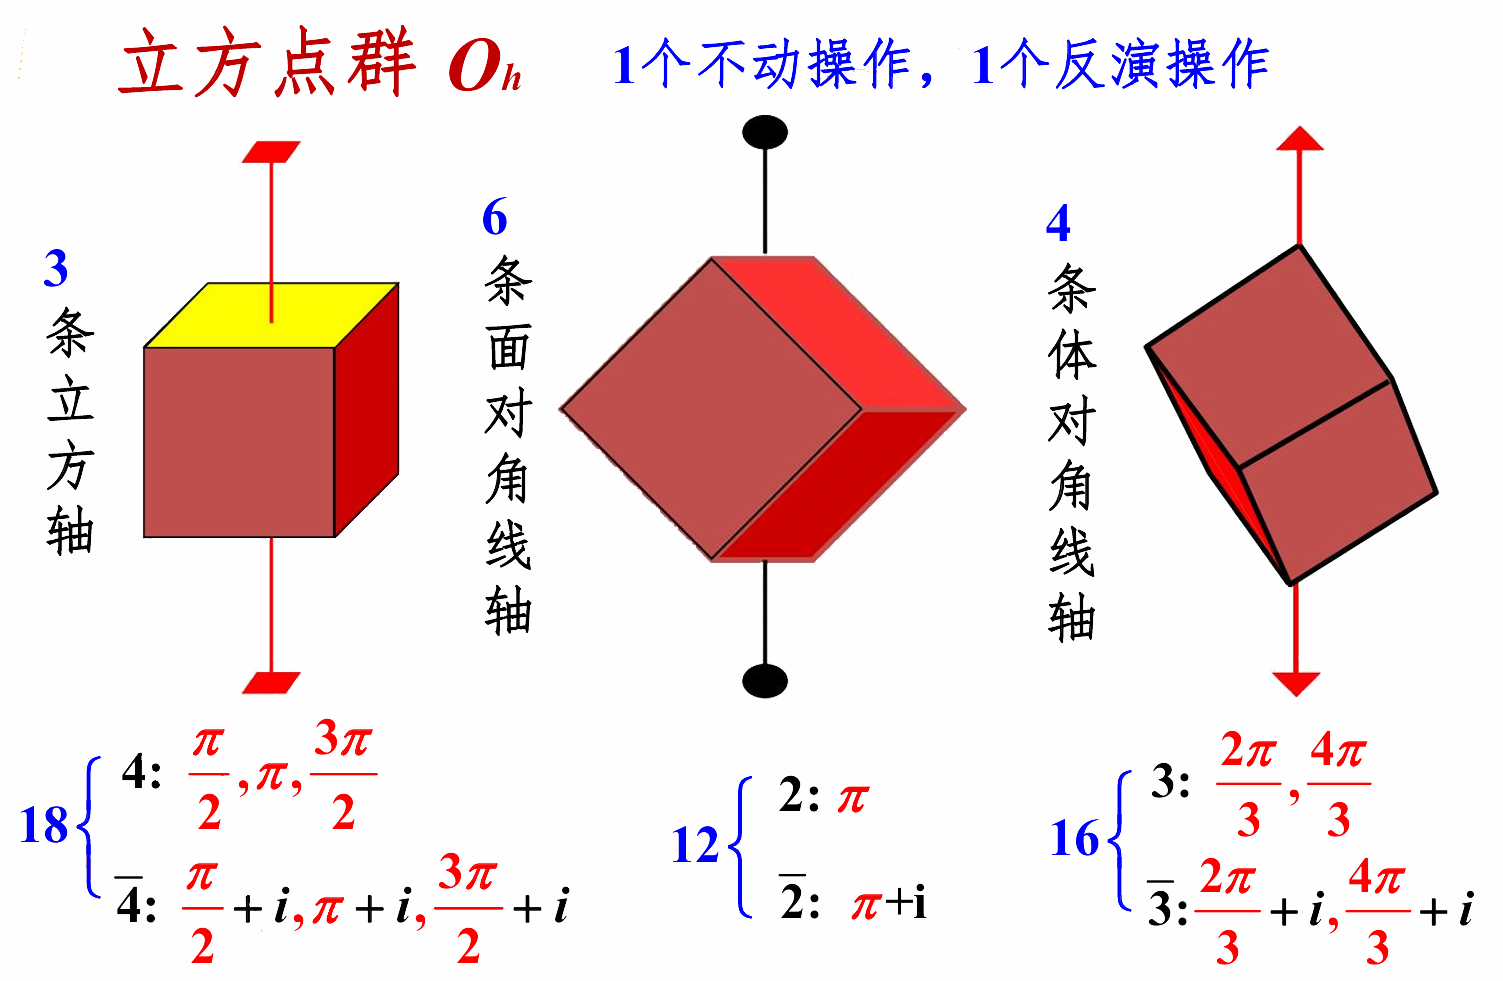
\includegraphics[height=20em, keepaspectratio=true]{pic/1-44}
        \caption{立方点群$O_h$的对称性}
        \label{fig:1-14}
    \end{figure}

    总结成表格形式,如\autoref{tab:1-11}所示:
    \begin{table}[!htbp]
        \centering
        \resizebox{\textwidth}{!}{
        \setlength{\tabcolsep}{1em}
        \begin{tabular}{clc}
            \toprule
            对称素                                    & 对称操作                                        & 数目 \\
            \midrule
            三个4重轴$\left\langle 100\right\rangle $ & 旋转$90^{\circ}$、$180^{\circ}$、$270^{\circ}$  & 9\\
            六个2重轴$\left\langle 110\right\rangle $ & 旋转$180^{\circ}$                               & 6\\
            四个3重轴$\left\langle 111\right\rangle $ & 旋转$120^{\circ}$、$240^{\circ}$                & 8\\
            \multirow{2}{*}{对称心}                   & 不动                                            & 1 \\
                                                      & 上述所有操作的反演                               & 24 \\
            \midrule
            \multicolumn{2}{c}{合计}                                                                   & 48 \\ 
            \bottomrule
        \end{tabular}
        }
        \caption{立方点群$O_h$的对称性}
        \label{tab:1-11}
    \end{table}

\subsubsection{正四面体点群$T_d$的对称性}
    我们考虑正四面体点群$T_d$的对称性。我们将正四面体点群$T_d$视为立方体点群$O_h$四个彼此不相邻的顶点,正四面体点群$T_d$的对称操作就包含在立方体点群$O_h$的对称操作之中。从而只需考虑正四面体点群$T_d$无法满足的对称操作即可。
    \begin{itemize}[itemsep=0pt,parsep=0pt]
        \item \textbf{不动与反演}:立方点群包括不动操作,不包括反演操作。
        \item \textbf{对于三条立方轴}:每根轴线作为4重旋转轴:包括绕立方轴旋转$180^{\circ}$;每根轴线作为4重旋转反演轴,包括绕立方轴旋转$90^{\circ}$、$270^{\circ}$再反演的三个对称操作。三条立方轴共计9个对称操作。
        \item \textbf{对于六条面对角线轴}:每根轴线作为2重旋转反演轴,包括绕面对角线轴旋转$180^{\circ}$再反演的一个对称操作。六条面对角线轴共计6个对称操作。
        \item \textbf{对于四条体对角线轴}:每根轴线作为4重旋转轴:包括绕立方轴旋转$120^{\circ}$、$240^{\circ}$的两个对称操作。四条面对角线轴共计8个对称操作。
    \end{itemize}
    综上,正四面体点群$T_d$共计$1+9+6+8=24$种对称操作,如\autoref{fig:1-15}所示:

    \begin{figure}[!htbp]
        \centering    
        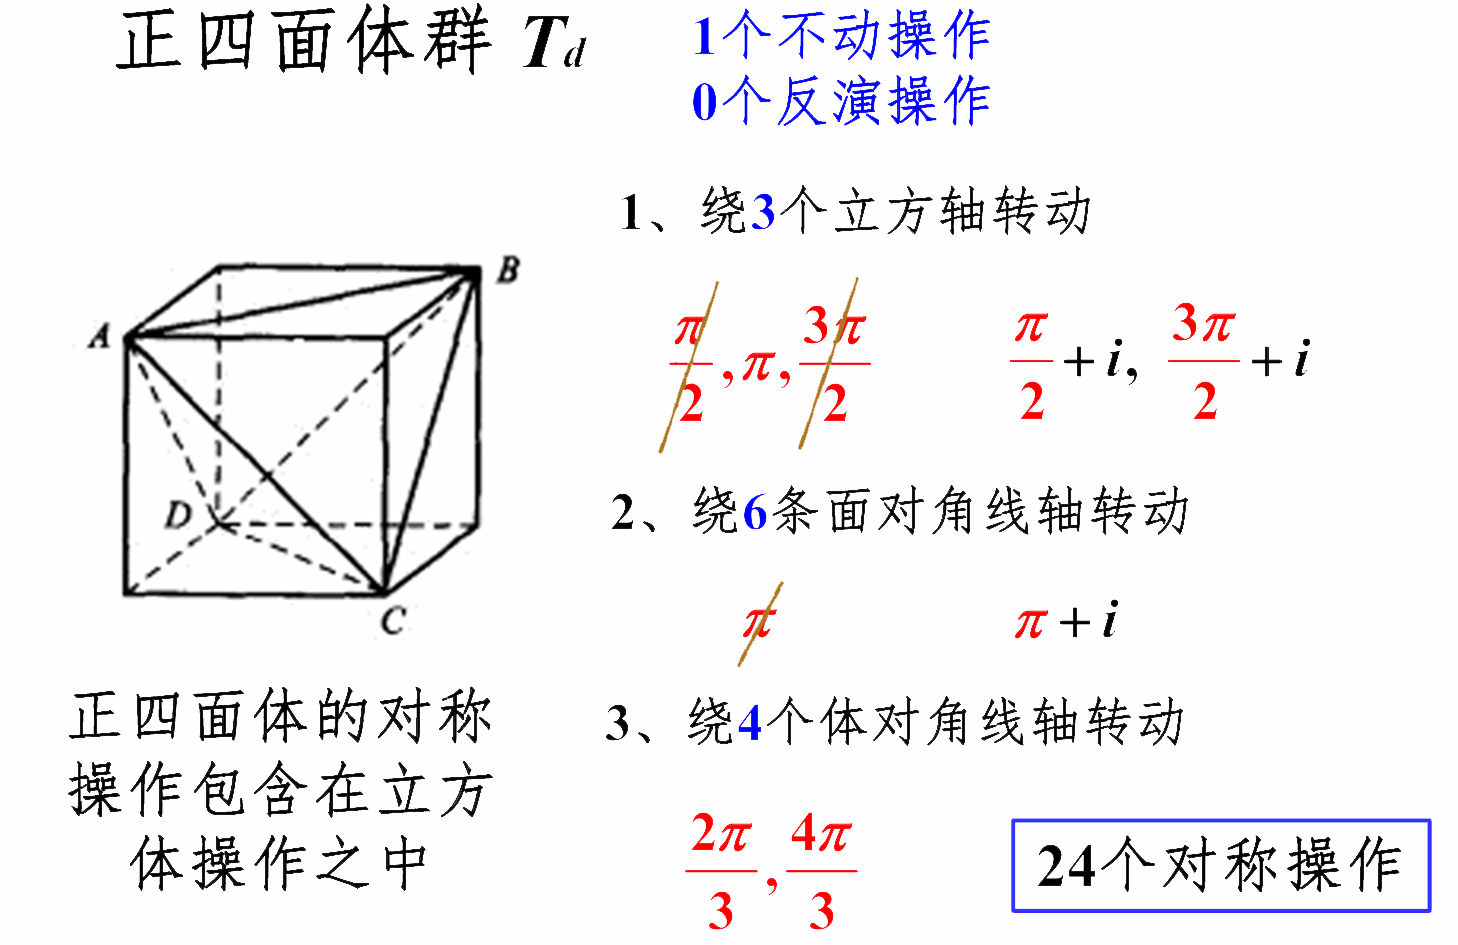
\includegraphics[height=20em, keepaspectratio=true]{pic/1-45}
        \caption{正四面体点群$T_d$的对称性}
        \label{fig:1-15}
    \end{figure}

    总结成表格形式,如\autoref{tab:1-12}所示。正四面体点群$T_d$是不具备反演及其对称心的,立方点群$O_h$所具备的4重轴和对称心$i$(即立方轴)退化为4重旋转反演轴,2重轴和对称心$i$(即面对角线)退化为2重旋转反演轴,3重轴和对称心$i$(即体对角线)退化为3重旋转轴,关于对称心的不动和反演退化为不动。因此立方点群$O_h$的对称性明显高于正四面体点群$T_d$。
    \begin{table}[!htbp]
        \centering
        \resizebox{\textwidth}{!}{
        \setlength{\tabcolsep}{1em}
        \begin{tabular}{clc}
            \toprule
            对称素                                           & 对称操作                                         & 数目 \\
            \midrule
            三条4重旋转反演轴$\left\langle 100\right\rangle $ & \makecell[l]{旋转$90^{\circ}$、$270^{\circ}$再反演,\\旋转$180^{\circ}$(反演两次复原)}  & 9\\
            六条2重旋转反演轴$\left\langle 110\right\rangle $ & 旋转$180^{\circ}$再反演                          & 6\\
            四条3重旋转轴$\left\langle 111\right\rangle $     & 旋转$120^{\circ}$、$240^{\circ}$                & 8\\
                                                             & 不动                                            & 1 \\
            \midrule
            \multicolumn{2}{c}{合计}                                                                           & 48 \\ 
            \bottomrule
        \end{tabular}
        }
        \caption{正四面体点群的对称性}
        \label{tab:1-12}
    \end{table}

\subsubsection{晶体的32种点群}
    由群论知识和晶格限制,晶体所具有的十种对称素$1,2,3,4,6,\overline{1},\overline{2},\overline{3},\overline{4},\overline{6}$只能构成32种点群,也就是说晶体的宏观对称性只有32种。
    
    应当指出,\nameref{tab:1-5}和\nameref{tab:1-6}的晶系是基于晶体的宏观对称性进行划分的的。一方面,这说明晶体的宏观对称性依然受到布拉菲格子乃至平移对称性的约束限制;另一方面,也反映布拉菲格子可以反映晶体的平移对称性与宏观对称性,是研究晶格的重要工具。

    综合考虑宏观对称性与平移对称性。点对称操作(旋转和反演)的集合构成点群,而平移对称操作(即平移晶格使晶体自身重合)的集合构成\textbf{平移群}。晶格全部对称操作,包括点对称操作和平移对称操作,其集合构成\textbf{空间群}。不同的空间群共230种。也就是说晶格结构的对称性共有230个类型。

\subsection{晶体宏观对称性的应用}
\subsubsection{物理性质张量}
    我们首先介绍\textbf{张量}\index{张量}的概念。\textbf{张量}(Tensor)是定义在向量空间和对偶空间的笛卡尔积上的多重线性映射,在$|n|$维空间内,含有$|n|$个分量,其中每个分量都是坐标的函数。在坐标变换时,这些分量也相应的作线性变换。

    张量概念包括标量、向量和线性算子,我们定义$r$为张量的\textbf{秩}或\textbf{阶数}\index{张量的阶数}。
    \begin{itemize}[itemsep=0pt,parsep=0pt]
        \item 第零阶张量$r = 0$为标量(Scalar)
        \item 第一阶张量$r = 1$为向量(Vector)
        \item 第二阶张量$r = 2$为矩阵(Matrix)
        \item 高阶张量$r \geq 3$可以作为线性算子,表述线性运算
    \end{itemize}

    物体的物理性质,常通过两个物理量之间的关系来定义。例如以下关系分别给出密度、电导率和介电常数:
    \begin{align*}
        m &= \rho \cdot V\\
        \vec{J} &= \sigma \cdot \vec{E}\\
        \vec{D} &= \varepsilon \cdot \vec{E}\\
    \end{align*}

    其一般形式为$B=C\cdot A$,其中$A$为$n$阶作用张量,$B$为$m$阶感生张量,$C$则为$m+n$阶物理性质张量。
    
    在三维笛卡尔空间中,$A$、$B$常为$1\times 3$的向量,即第一阶张量$r=1$。于是可以用$3\times 3$的矩阵,即第二阶张量$r=2$表述物理性质张量$C$:
    \[
    C=
    \left(
    \begin{array}{ccc}
        c_{11} & c_{12} & c_{13} \\
        c_{21} & c_{22} & c_{23} \\
        c_{31} & c_{32} & c_{33} \\
    \end{array}
    \right)
    \]

\subsubsection{诺埃曼原理和居里原理}
    诺埃曼原理和居里原理分别不存在外场作用和存在外场作用时,晶体物理性质张量$C$的对称性与晶体宏观对称性的关系。

    \textbf{诺埃曼原理}\index{诺埃曼原理}:晶体物理性质的对称性$\geq$晶体的宏观对称性。

    \textbf{居里原理}\index{居里原理}:晶体所受外场作用的对称性$\geq$晶体的宏观对称性。即当晶体所受外场作用的对称性$\geq$晶体原本的宏观对称性时,晶体宏观对称性不变;当晶体所受外场作用的对称性$<$晶体原本的宏观对称性时,晶体宏观对称性被迫降低。

    我们可以认为:居里原理考察外场作用与晶体宏观对称性的关系;而诺埃曼原理则考察晶体物理性质与晶体宏观对称性的关系。当外场作用不得忽略时,需要先利用居里原理确定晶体的宏观对称性,外场作用后晶体的物理性质与晶体此时的宏观对称性依然满足诺埃曼原理。

    这就说明,我们可以利用晶体的宏观对称性对晶体的物理性质张量$C$做出限制与约束,从而简化其运算或形式。我们考虑下面的例子。

    对于晶体的介电常数,我们有:
    \[
    \vec{D} = \boldsymbol{\varepsilon} \cdot \vec{E}
    \]
    其中介电常数$\boldsymbol{\varepsilon}$用矩阵表示为:
    \[
    \boldsymbol{\varepsilon}=
    \left(
    \begin{array}{ccc}
        \varepsilon_{11} & \varepsilon_{12} & \varepsilon_{13} \\
        \varepsilon_{21} & \varepsilon_{22} & \varepsilon_{23} \\
        \varepsilon_{31} & \varepsilon_{32} & \varepsilon_{33} \\
    \end{array}
    \right)
    \]

    对晶体进行旋转操作,我们回忆旋转操作的变换矩阵:
    \[
    A=
    \left(
    \begin{array}{ccc}
        \cos\theta & -\sin\theta & 0 \\
        \sin\theta & \cos\theta  & 0 \\
        0          & 0           & 1 
    \end{array}
    \right)
    \]
    应注意$A$是正交矩阵,由正交性$A^T=A^{-1}$。

    旋转操作后,电位移矢量与电场强度发生改变,有:
    \begin{align*}
        \vec{D'} &= A \cdot \vec{D}\\
        \vec{E'} &= A \cdot \vec{E}
    \end{align*}

    介电常数可以相应的表示为:
    \[
    \vec{D'} = \boldsymbol{\varepsilon'} \cdot \vec{E'}
    \]

    联立可得:
    \begin{align*}
        \vec{D'}= \boldsymbol{\varepsilon'} \cdot \vec{E'}&= A \cdot \vec{D}\\
                                                          &= A \cdot \boldsymbol{\varepsilon} \cdot \vec{E}\\
                                                          &= A \cdot \boldsymbol{\varepsilon} \cdot A^{-1} \cdot \vec{E'}
    \end{align*}

    旋转不改变介电常数本身,即介电常数矩阵$\boldsymbol{\varepsilon}$满足
    \begin{align*}
        \boldsymbol{\varepsilon'} &= A \cdot \boldsymbol{\varepsilon} \cdot A^{-1}\\
                                  &= A \cdot \boldsymbol{\varepsilon} \cdot A^{T} = \boldsymbol{\varepsilon} 
    \end{align*}

    这体现了晶体的介电常数这一物理性质,其张量$\boldsymbol{\varepsilon}$的分量受到旋转矩阵$A$的约束与限制,因此晶体的宏观对称性大大减少了独立分量数目。即:\textbf{晶体的对称性在确定晶体物理常数的独立个数上有重要意义,它可以简化物理常数的测量。}

    我们以立方晶体、六角对称晶体为例,它们各自具有关于$90^{\circ}$和$60^{\circ}$的旋转不变性。我们接下来将看到晶体各自的宏观对称性是如何简化物理性质张量的。

    \newpage
    \begin{itemize}[itemsep=0pt,parsep=0pt]
        \item \textbf{立方对称的晶体}:在立方对称的晶体中,我们选取两次旋转操作:
        \begin{itemize}[itemsep=0pt,parsep=0pt]
            \item 
            绕4重旋转轴($z$轴)旋转$90^{\circ}$,旋转矩阵$
            A=
            \left(
            \begin{array}{ccc}
                0 & -1 & 0 \\
                1 & 0 & 0 \\
                0 & 0 & 1 
            \end{array}
            \right)
            $

            \begin{align*}
                A \cdot \boldsymbol{\varepsilon} \cdot A^{T}&=
                \left(
                \begin{array}{ccc}
                    0 & -1 & 0 \\
                    1 & 0 & 0 \\
                    0 & 0 & 1 
                \end{array}
                \right)
                \cdot
                \left(
                \begin{array}{ccc}
                    \varepsilon_{11} & \varepsilon_{12} & \varepsilon_{13} \\
                    \varepsilon_{21} & \varepsilon_{22} & \varepsilon_{23} \\
                    \varepsilon_{31} & \varepsilon_{32} & \varepsilon_{33} \\
                \end{array}
                \right)
                \cdot
                \left(
                \begin{array}{ccc}
                    0 & 1 & 0 \\
                    -1 & 0 & 0 \\
                    0 & 0 & 1 
                \end{array}
                \right)\\
                &=
                \left(
                \begin{array}{ccc}
                    \varepsilon_{22} & -\varepsilon_{21} & -\varepsilon_{23} \\
                    -\varepsilon_{12} & \varepsilon_{11} & \varepsilon_{13} \\
                    -\varepsilon_{32} & \varepsilon_{31} & \varepsilon_{33} \\
                \end{array}
                \right)
                \equiv 
                \left(
                \begin{array}{ccc}
                    \varepsilon_{11} & \varepsilon_{12} & \varepsilon_{13} \\
                    \varepsilon_{21} & \varepsilon_{22} & \varepsilon_{23} \\
                    \varepsilon_{31} & \varepsilon_{32} & \varepsilon_{33} \\
                \end{array}
                \right)
                =\boldsymbol{\varepsilon}
            \end{align*}
            化简可得
            \[
            \boldsymbol{\varepsilon}=
            \left(
            \begin{array}{ccc}
                \varepsilon_{0} & 0 & 0 \\
                0 & \varepsilon_{0} & 0 \\
                0 & 0 & \varepsilon_{33} \\
            \end{array}
            \right)
            \]
            \item
            绕4重旋转轴($x$轴)旋转$90^{\circ}$,旋转矩阵$ 
            A=
            \left(
            \begin{array}{ccc}
                1 & 0 & 0 \\
                0 & 0 & -1\\
                0 & 1 & 0
            \end{array}
            \right)
            $

            \begin{align*}
                A \cdot \boldsymbol{\varepsilon} \cdot A^{T}&=
                \left(
                \begin{array}{ccc}
                    1 & 0 & 0 \\
                    0 & 0 & -1\\
                    0 & 1 & 0
                \end{array}
                \right)
                \cdot
                \left(
                \begin{array}{ccc}
                    \varepsilon_{0} & 0 & 0 \\
                    0 & \varepsilon_{0} & 0 \\
                    0 & 0 & \varepsilon_{33} \\
                \end{array}
                \right)
                \cdot
                \left(
                \begin{array}{ccc}
                    1 & 0 & 0 \\
                    0 & 0 & 1 \\
                    0 & -1 & 0
                \end{array}
                \right)\\
                &=
                \left(
                \begin{array}{ccc}
                    \varepsilon_{0} & 0 & 0 \\
                    0 & \varepsilon_{0} & 0 \\
                    0 & 0 & \varepsilon_{0}
                \end{array}
                \right)
                \equiv \boldsymbol{\varepsilon}
            \end{align*}
        \end{itemize}
        综上可知,立方对称的晶体的介电常数$\boldsymbol{\varepsilon}$用矩阵表示为:
        \[
        \boldsymbol{\varepsilon}=
        \left(
        \begin{array}{ccc}
            \varepsilon_{0} & 0 & 0 \\
            0 & \varepsilon_{0} & 0 \\
            0 & 0 & \varepsilon_{0} \\
        \end{array}
        \right)
        \]
        这实际上是一个标量,即\textbf{立方对称的晶体的介电常数为标量}。

        \item \textbf{六角对称的晶体}:在六角对称的晶体中,我们绕6重旋转对称轴($z$轴)旋转$60^{\circ}$,旋转矩阵$ 
        A=
        \left(
        \begin{array}{ccc}
            \frac{1}{2} & -\frac{\sqrt{3}}{2} & 0 \\
            \frac{\sqrt{3}}{2} & \frac{1}{2} & 0 \\
            0 & 0 & 1
        \end{array}
        \right)
        $
        
        \begin{align*}
                &A \cdot \boldsymbol{\varepsilon} \cdot A^{T}=
                \left(
                \begin{array}{ccc}
                    \frac{1}{2} & -\frac{\sqrt{3}}{2} & 0 \\
                    \frac{\sqrt{3}}{2} & \frac{1}{2} & 0 \\
                    0 & 0 & 1
                \end{array}
                \right)
                \cdot
                \left(
                \begin{array}{ccc}
                    \varepsilon_{11} & \varepsilon_{12} & \varepsilon_{13} \\
                    \varepsilon_{21} & \varepsilon_{22} & \varepsilon_{23} \\
                    \varepsilon_{31} & \varepsilon_{32} & \varepsilon_{33} \\
                \end{array}
                \right)
                \cdot
                \left(
                \begin{array}{ccc}
                    \frac{1}{2} & \frac{\sqrt{3}}{2} & 0 \\
                    -\frac{\sqrt{3}}{2} & \frac{1}{2} & 0 \\
                    0 & 0 & 1
                \end{array}
                \right)\\
                &=
                \left(
                \begin{array}{ccc}
                \frac{1}{4}\varepsilon_{11}-\frac{3}{4}\varepsilon_{22}+\tfrac{\sqrt{3}}{4}(\varepsilon_{12}-\varepsilon_{21}) &
                -\tfrac{\sqrt{3}}{4}\varepsilon_{11}+\tfrac{1}{4}\varepsilon_{12}+\tfrac{3}{4}\varepsilon_{21}-\tfrac{\sqrt{3}}{4}\varepsilon_{22} &
                \tfrac{1}{2}\varepsilon_{13}-\tfrac{\sqrt{3}}{2}\varepsilon_{23}
                \\[8pt]
                \tfrac{\sqrt{3}}{4}\varepsilon_{11}+\tfrac{3}{4}\varepsilon_{12}+\tfrac{1}{4}\varepsilon_{21}+\tfrac{\sqrt{3}}{4}\varepsilon_{22} &
                -\tfrac{3}{4}\varepsilon_{11}+\tfrac{1}{4}\varepsilon_{22}+\tfrac{\sqrt{3}}{4}(\varepsilon_{12}-\varepsilon_{21}) &
                \tfrac{\sqrt{3}}{2}\varepsilon_{13}+\tfrac{1}{2}\varepsilon_{23}
                \\[8pt]
                \tfrac{1}{2}\varepsilon_{31}+\tfrac{\sqrt{3}}{2}\varepsilon_{32} &
                -\tfrac{\sqrt{3}}{2}\varepsilon_{31}+\tfrac{1}{2}\varepsilon_{32} &
                \varepsilon_{33}
                \end{array}
                \right)\\
                &\equiv \boldsymbol{\varepsilon}=
                \left(
                \begin{array}{ccc}
                    \varepsilon_{11} & \varepsilon_{12} & \varepsilon_{13} \\
                    \varepsilon_{21} & \varepsilon_{22} & \varepsilon_{23} \\
                    \varepsilon_{31} & \varepsilon_{32} & \varepsilon_{33} \\
                \end{array}
                \right)
        \end{align*}
        通过矩阵求解方程,我们可以整理得到:
        \[
        \boldsymbol{\varepsilon}=
        \left(
        \begin{array}{ccc}
            \varepsilon_{\perp } & 0 & 0 \\
            0 & \varepsilon_{\perp } & 0 \\
            0 & 0 & \varepsilon_{\mathop{//}} \\
        \end{array}
        \right)
        \]

        介电常数在平行于$z$轴与垂直于$z$轴方向上的差别,正是六角对称晶体具有双折射现象的成因。
    \end{itemize}

\section{晶体的结合}
    \textbf{晶体的结合}\index{晶体的结合}有四种基本方式:
    \begin{itemize}[itemsep=0pt,parsep=0pt]
        \item \textbf{离子型}:正、负离子间的静电吸引力
        \item \textbf{金属型}:离子实与价电子之间的静电库仑力
        \item \textbf{共价型}:最外层电子不会脱离原来原子,靠近的两原子各出一个电子,形成电子共享。这一对电子的自旋相反,称为配对电子。
        \item \textbf{范德华型}:源自瞬时偶极与诱导偶极之间的弱相互作用,结合力较弱。
    \end{itemize}
    实际晶体的结合以这四种方式为基础,可能同时包含上述的多种方式。

\chapter{倒格子与波矢空间}\label{chap:2}
    本章将利用傅里叶变换,从晶格和布拉菲点阵所处的位置空间,进入波矢和倒格子所处的波矢空间:
    \[
        \mbox{<位置空间>}\xrightarrow{\mbox{傅里叶变换}}\mbox{<波矢空间>} 
    \]

    我们通过\autoref{fig:1-16}的例子,来说明傅里叶变换的核心思想。对于时域的方波信号,经过傅里叶变换得到其不同频率的正余弦分量,并以这些频率分量$k$为参数绘制频域,从而将时域信号转换为频域分量。即对于同一物理问题,通过不同视角,可以使问题得到简化。

    \begin{figure}[!htbp]
        \centering    
        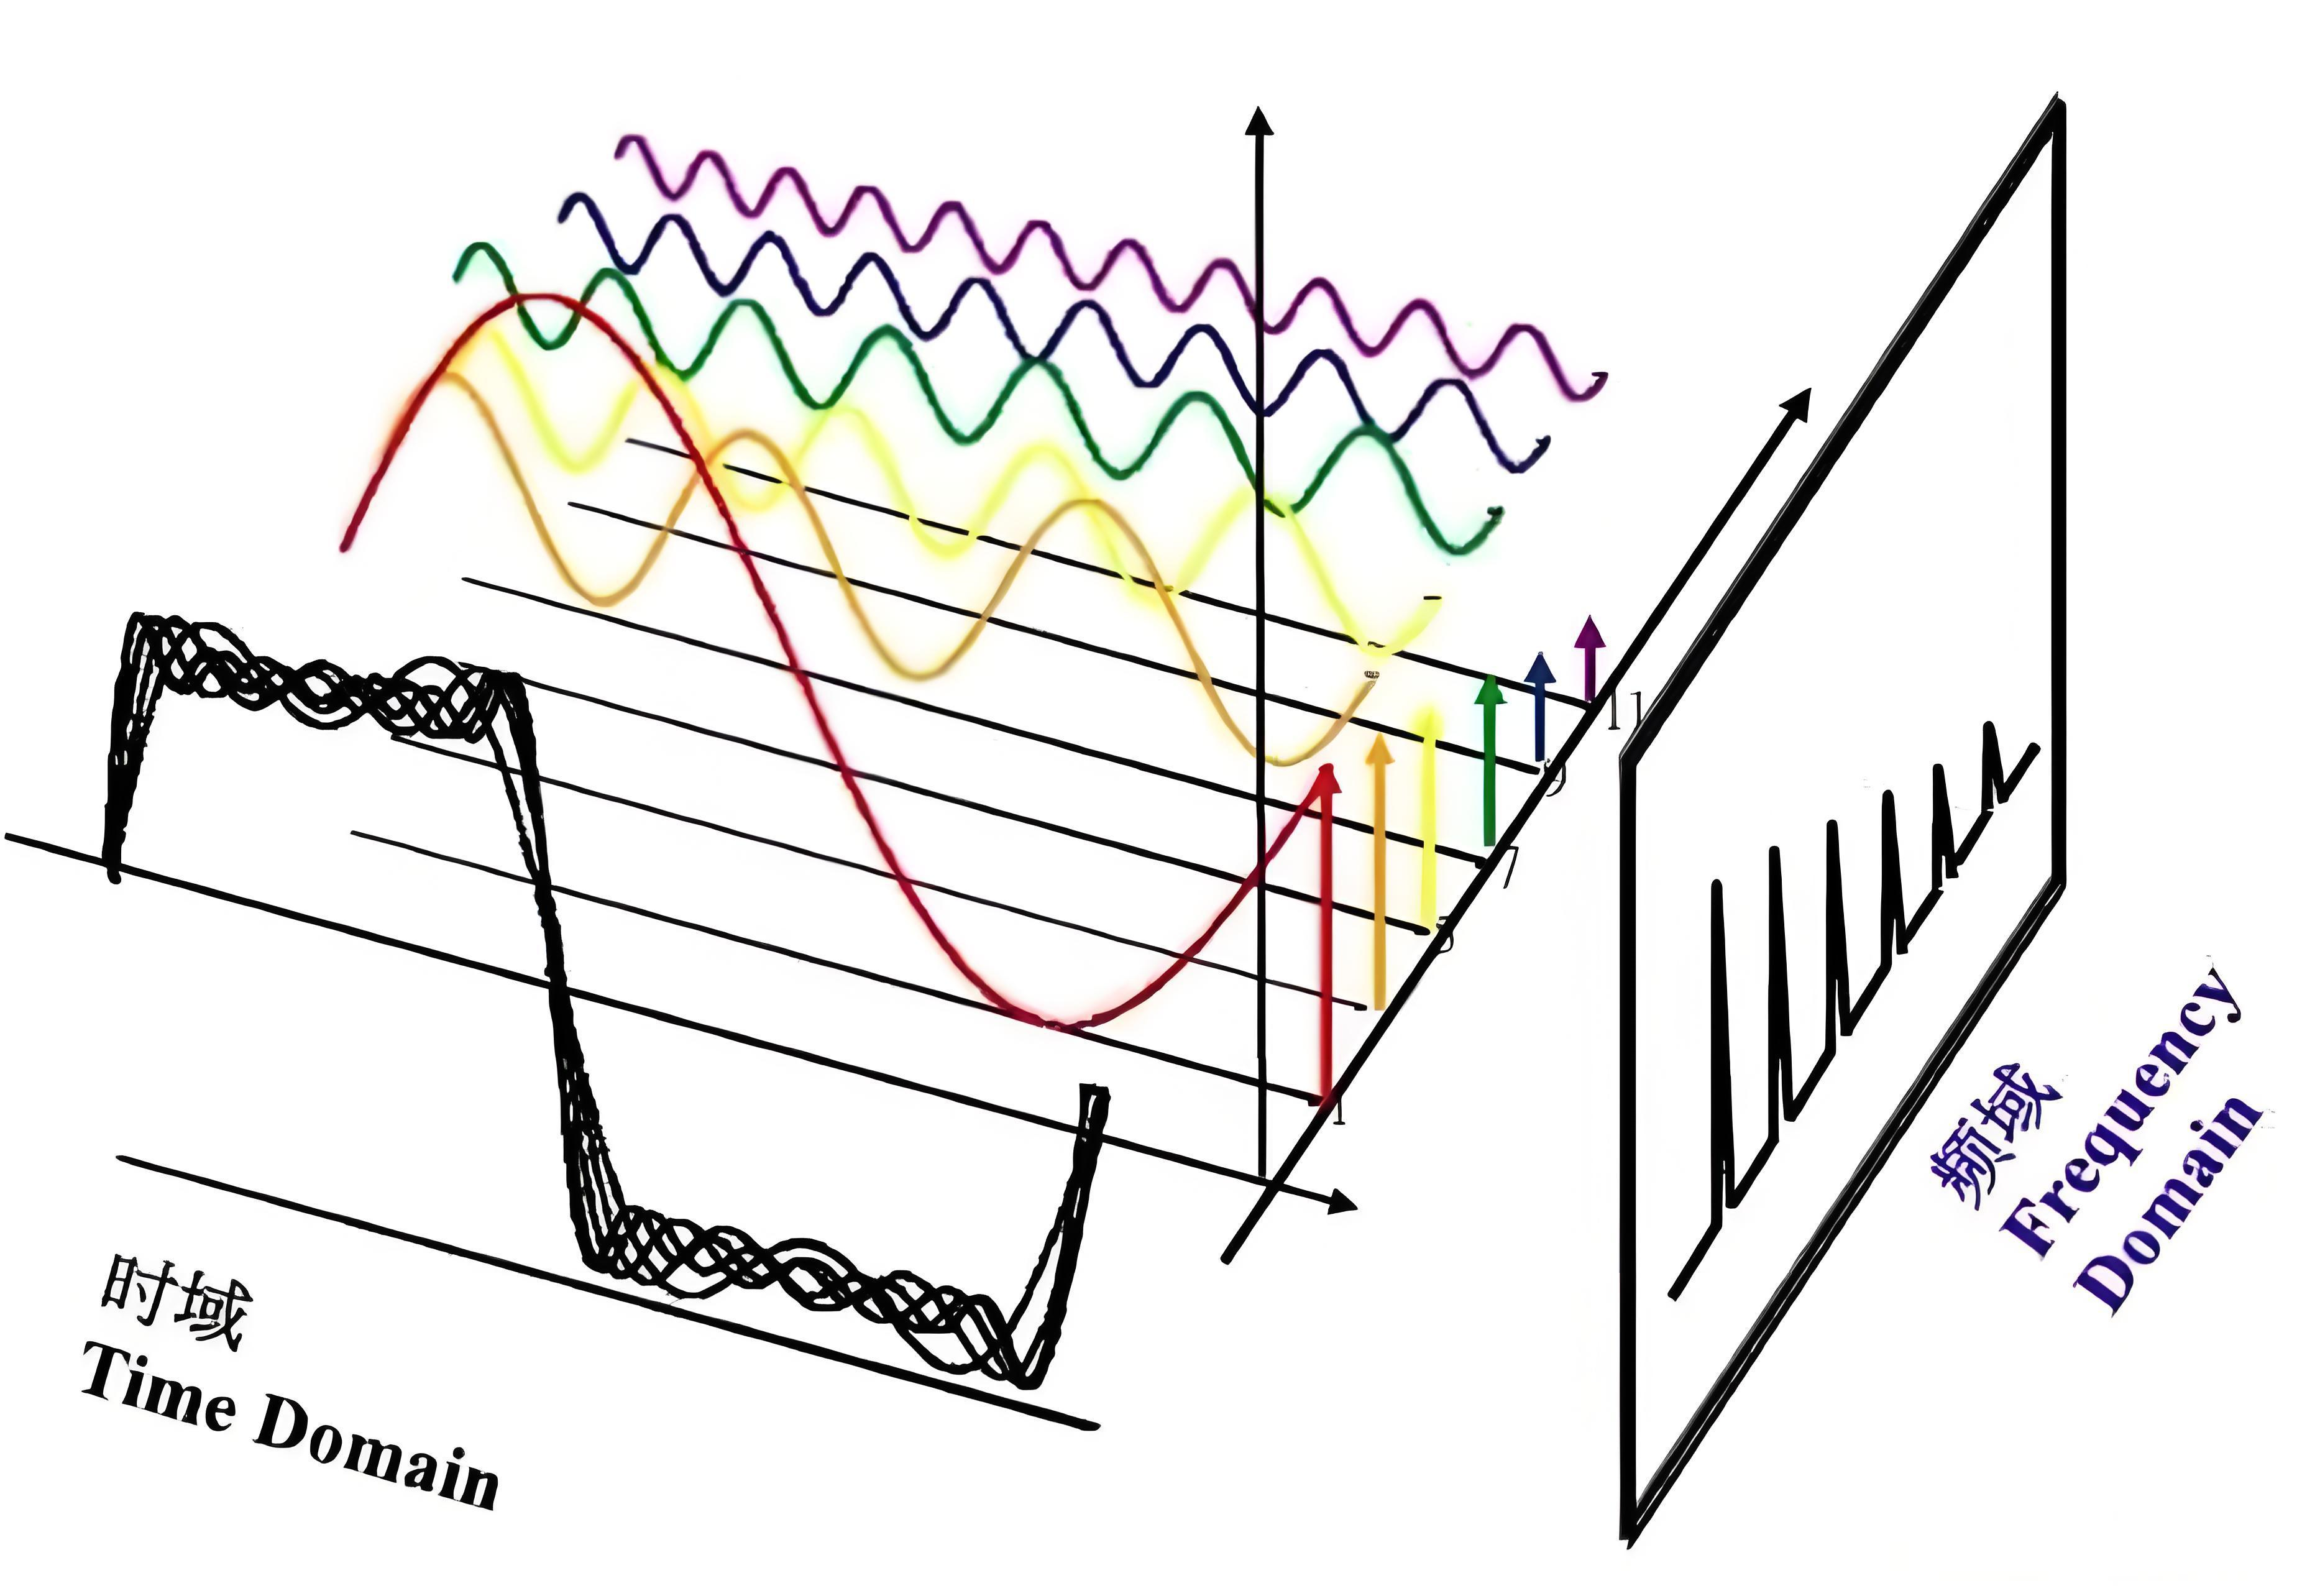
\includegraphics[height=8em, keepaspectratio=true]{pic/2-01}
        \caption{傅里叶变换的核心思想}
        \label{fig:1-16}
    \end{figure}

    傅里叶变换表征所包含的不同频率的正/余弦波的振幅,其公式如下:
    \begin{align}
        F(k)&=\frac{1}{\sqrt{2\pi}}\int_{-\infty}^{+\infty} f(x)e^{-jkx} \,\mathrm{d}x\\
        f(x)&=\frac{1}{\sqrt{2\pi}}\int_{-\infty}^{+\infty} F(k)e^{+jkx} \,\mathrm{d}k 
    \end{align}
           
    应用傅里叶变换,可以方便地研究晶格中波的传播与相互作用。我们重点关注晶格中的这三种波:
    \begin{itemize}[itemsep=0pt,parsep=0pt]
        \item \textbf{X射线衍射的电磁波}:X射线、中子、电子束在晶体中的衍射是研究晶体结构最重要的手段。
        \item \textbf{晶格振动的格波}:晶体中的原子并非静止不动,而是在平衡位置附近振动。这种振动以波的形式在晶体中传播。原子集体的振动模式被称为格波,每一种振动模式都可以看作一种简谐波。
        \item \textbf{电子的物质波}:电子具有波粒二象性,其量子态用一个波函数来描述。自由电子的波函数表现为行波;晶体中的电子处在原子核周期性排列产生的势场中,波函数更加复杂。
    \end{itemize}

    我们将在本章最后\nameref{sec:2-3}介绍X射线衍射探测晶格,并作为倒格子的一种应用;随后在\nameref{chap:3}介绍晶格振动所产生的格波、在\nameref{chap:4}介绍电子的德布罗意波。而实际上,X射线的电磁波需要与晶格的格波发生相互作用才能显示结构、电子在晶体中的运动也是电子的德布罗意波与晶格的格波相互作用的结果。
    
\section{倒格子}
\subsection{倒映空间}
    将在坐标空间的点阵,即布拉菲格子,称为\textbf{正格子}\index{正格子}。

    如\nameref{tag:Crystal_Periodicity}所述,晶体内的任意物理量$V(\vec{r})$都是关于平移矢量$\vec{R}$的周期函数。即:
    \begin{equation}
        V(\vec{r})=V(\vec{r}+\vec{R})
    \end{equation}

    两边同时做傅里叶变换有:

    \begin{equation}
    \begin{aligned}
        \frac{1}{\sqrt{2\pi}}\int_{-\infty}^{+\infty} V(\vec{r})e^{-j\vec{k}\vec{r}} \,\mathrm{d}\vec{r}&=\frac{1}{\sqrt{2\pi}}\int_{-\infty}^{+\infty} V(\vec{r}+\vec{R})e^{-j\vec{k}(\vec{r}+\vec{R})} \,\mathrm{d}\vec{r}\\
        &=\frac{1}{\sqrt{2\pi}}\int_{-\infty}^{+\infty} V(\vec{r})e^{-j\vec{k}\vec{r}}\cdot e^{-j\vec{k}\vec{R}} \,\mathrm{d}\vec{r}
    \end{aligned}
    \end{equation}
    其中$\vec{k}$为波矢,作为傅里叶变换后波矢空间的参数。

    为使等号成立,要求
    \begin{equation}
        e^{-j\vec{k}\vec{R}}=1\qquad\mbox{即:}\vec{k}\cdot\vec{R}=2\pi n
    \end{equation}
    其中$n$取整数,$n=\dots{-2},-1,0,1,2\dots$

    坐标空间的原胞的平移矢量写为$\vec{R}=l_1\vec{a_1}+l_2\vec{a_2}+l_3\vec{a_3}$,其中$\vec{a_i}$为原胞对应方向的晶格基矢;类似的,我们定义晶格中的任意波矢$\vec{k}=k_1\vec{b_1}+k_2\vec{b_2}+k_3\vec{b_3}$,其中$\vec{b_j}$为波矢空间中的基矢,称为\textbf{倒格矢}\index{倒格矢},且$a_i$、$b_j$满足:

    \begin{equation}\label{eq:2.6}
        \vec{a_i}\cdot\vec{b_j}=
        \begin{cases}
            2\pi,&i=j\\
            0,&i\neq j
        \end{cases}
        =2\pi\delta_{ij}
    \end{equation}

    在三维笛卡尔空间中,倒格矢$\vec{b_i}$与另外两个晶格基矢$\vec{a_j}$、$\vec{a_k}$正交,其单位是$\frac{2\pi}{\mbox{[长度]}}$。倒格子依然是结点的有序排列,从点阵的角度,倒格子同样属于布拉菲点阵,也就自然只有7种晶系、十四种布拉菲格子。

    正格子与倒格子的归纳如\autoref{tab:1-13}所示:
    \begin{table}[!htbp]
        \centering
        \setlength{\tabcolsep}{1em}
        \begin{tabular}{cc}
            \toprule
            \multicolumn{2}{c}{\textbf{布拉菲点阵}}\\
            \multicolumn{2}{c}{5种二维布拉菲点阵/14种三维布拉菲格子}\\
            \midrule
            \textbf{坐标空间}           & \textbf{倒映空间}\\
            晶格                        & 倒格子\\
            反映晶体的空间结构           & 反映晶体的物理性质\\
            \midrule
            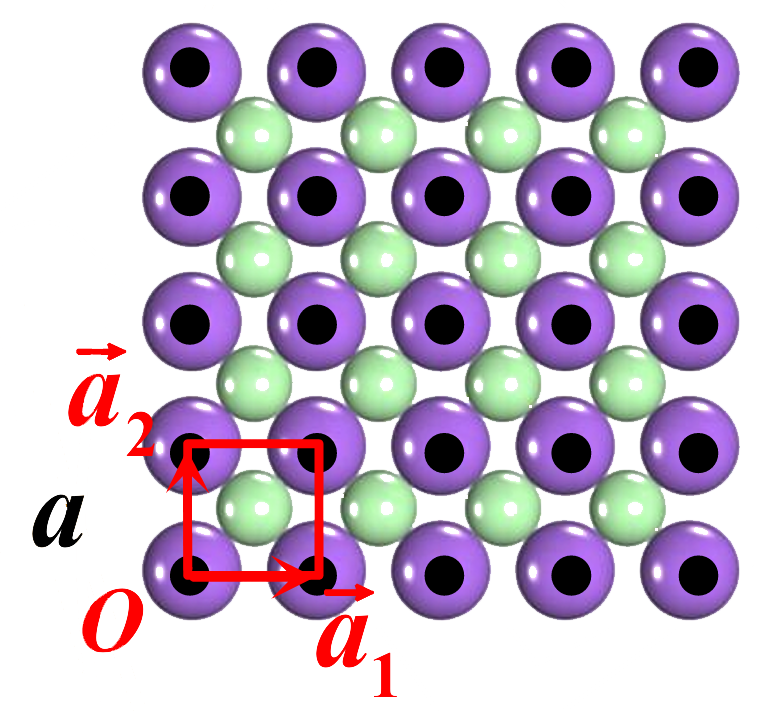
\includegraphics[valign=m, height=5em, keepaspectratio=true]{pic/2-02}&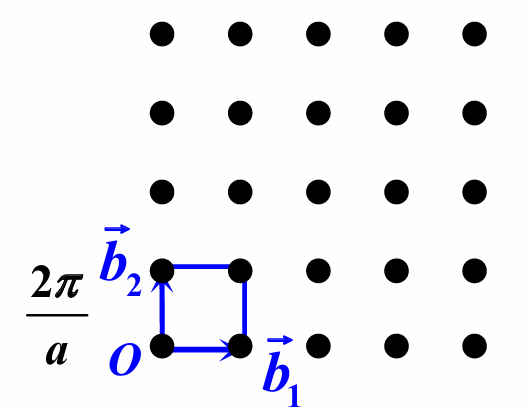
\includegraphics[valign=m, height=5em, keepaspectratio=true]{pic/2-03}\\
            \bottomrule
        \end{tabular}
        \caption{正格子与倒格子}
        \label{tab:1-13}
    \end{table}

\subsection{倒格矢的确定}
    本节则从\autoref{eq:2.6}出发,介绍如何确定二维倒格矢与三维倒格矢,并给出常见点阵的倒格矢。
\subsubsection{二维倒格矢的确定}
    在二维点阵中重述\autoref{eq:2.6}有:
    \begin{subequations}\label{eq:2.7}
    \begin{align}
        \vec{b_1} \cdot \vec{a_1} &= 2\pi\\
        \vec{b_1} \cdot \vec{a_2} &= 0
    \end{align}
    \end{subequations}
    我们只考虑了一个方向的倒格矢$\vec{b_1}$,另一个方向的倒格矢$\vec{b_2}$同理。

    想确定矢量就是要确定其模值与方向,而\autoref{eq:2.7}的两个式子就分别确定了模值与方向:
    \begin{itemize}[itemsep=0pt,parsep=0pt]
        \item 对于$\vec{b_1} \cdot \vec{a_2} = 0$,可知倒格矢$\vec{b_1}$与晶格基矢$\vec{a_2}$正交,倒格矢$\vec{b_1}$的方向垂直于晶格基矢$\vec{a_2}$;
        \item 对于$\vec{b_1} \cdot \vec{a_1} = 2\pi$,可知晶格基矢$\vec{a_1}$在倒格矢$\vec{b_1}$方向上的投影,与倒格矢$\vec{b_1}$模值的乘积,等于$2\pi$。
    \end{itemize}
    从而倒格矢$\vec{b_1}$得到确定。

    \nameref{tab:1-5}中的长方晶格、六角晶格的倒格矢如\autoref{fig:1-17}所示:
    \begin{figure}[!htbp]
        \centering    
        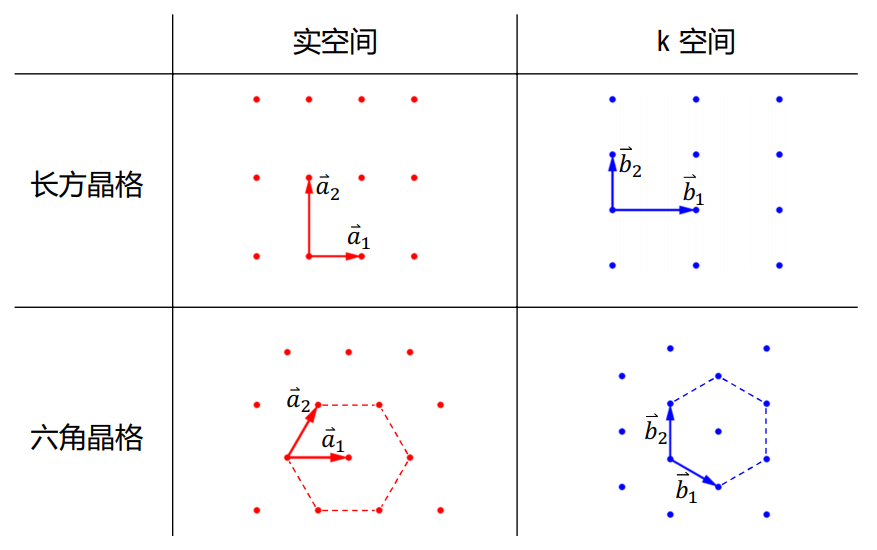
\includegraphics[height=14em, keepaspectratio=true]{pic/2-04}
        \caption{二维倒格矢的确定}
        \label{fig:1-17}
    \end{figure}

\subsubsection{三维倒格矢的确定}
    在三维点阵中重述\autoref{eq:2.6}有:
    \begin{subequations}\label{eq:2.8}
    \begin{align}
        \vec{b_1} \cdot \vec{a_1} &= 2\pi\\
        \vec{b_1} \cdot \vec{a_2} &= 0\\
        \vec{b_1} \cdot \vec{a_3} &= 0
    \end{align}
    \end{subequations}
    对于倒格矢$b_2$、$b_3$同理。

    依然从方向与模值的角度进行考虑\autoref{eq:2.8}:
    \begin{itemize}[itemsep=0pt,parsep=0pt]
        \item 对于$\vec{b_1} \cdot \vec{a_2} = 0$和$\vec{b_1} \cdot \vec{a_3} = 0$,可知倒格矢$\vec{b_1}$与晶格基矢$\vec{a_2}$、$\vec{a_3}$正交,倒格矢$\vec{b_1}$的方向垂直于晶格基矢$\vec{a_2}$与$\vec{a_2}$所确定的平面。如果记晶格基矢$\vec{a_2}$与$\vec{a_2}$所确定的平面的法向量为$\vec{e_n}=\vec{a_2} \times \vec{a_3}$,则有$\vec{b_1}\mathop{//}\vec{e_n}$;
        \item 对于$\vec{b_1} \cdot \vec{a_1} = 2\pi$,可知晶格基矢$\vec{a_1}$在法向量$\vec{e_n}=\vec{a_2} \times \vec{a_3}$方向上的投影,与倒格矢$\vec{b_1}$模值的乘积,等于$2\pi$。
    \end{itemize}
    从而倒格矢$\vec{b_1}$得到确定。

    为了方便计算,整理三维倒格矢的公式如下:
    \begin{equation}\label{eq:2.9}
    \begin{aligned}
        \vec{b_1} &=2\pi\frac{\vec{a_2}\times\vec{a_3}}{\vec{a_1}\cdot(\vec{a_2}\times\vec{a_3})}\\
        \vec{b_2} &=2\pi\frac{\vec{a_3}\times\vec{a_1}}{\vec{a_2}\cdot(\vec{a_3}\times\vec{a_1})}\\
        \vec{b_3} &=2\pi\frac{\vec{a_1}\times\vec{a_2}}{\vec{a_3}\cdot(\vec{a_1}\times\vec{a_2})}
    \end{aligned}
    \end{equation}

    \begin{table}[!htbp]
        \centering
        \resizebox{\textwidth}{!}{
        \setlength{\tabcolsep}{1em}
        \begin{tabular}{cclcl}
            \toprule
            晶格类型 & \multicolumn{2}{c}{原胞基矢} & \multicolumn{2}{c}{倒格矢}\\
            \midrule
            面心立方 & \includegraphics[valign=m, height=3em, keepaspectratio=true]{pic/1-25} & $
            \begin{cases}
            \vec{a_1}=\frac{a}{2}(\vec{i}+\vec{j})\\
            \vec{a_2}=\frac{a}{2}(\vec{j}+\vec{k})\\
            \vec{a_3}=\frac{a}{2}(\vec{k}+\vec{i})\\
            \end{cases}
            $ & \includegraphics[valign=m, height=3em, keepaspectratio=true]{pic/1-26} & $
            \begin{cases}
            \vec{b_1}=\frac{2\pi}{a}(\vec{i}+\vec{j}-\vec{k})\\
            \vec{b_2}=\frac{2\pi}{a}(\vec{j}+\vec{k}-\vec{i})\\
            \vec{b_3}=\frac{2\pi}{a}(\vec{k}+\vec{i}-\vec{j})\\
            \end{cases}
            $ \\
            体心立方 & \includegraphics[valign=m, height=3em, keepaspectratio=true]{pic/1-26} & $
            \begin{cases}
            \vec{a_1}=\frac{a}{2}(\vec{i}+\vec{j}-\vec{k})\\
            \vec{a_2}=\frac{a}{2}(\vec{j}+\vec{k}-\vec{i})\\
            \vec{a_3}=\frac{a}{2}(\vec{k}+\vec{i}-\vec{j})\\
            \end{cases}
            $ & \includegraphics[valign=m, height=3em, keepaspectratio=true]{pic/1-26} & $
            \begin{cases}
            \vec{b_1}=\frac{2\pi}{a}(\vec{i}+\vec{j})\\
            \vec{b_2}=\frac{2\pi}{a}(\vec{j}+\vec{k})\\
            \vec{b_3}=\frac{2\pi}{a}(\vec{k}+\vec{i})\\
            \end{cases}
            $ \\
            \bottomrule
        \end{tabular}
        }
        \caption{面心立方与体心立方的倒格矢}
        \label{tab:1-14}
    \end{table}

    \autoref{tab:1-14}考虑面心立方与体心立方的倒格矢,可以发现:面心立方与体心立方互为倒格子。

\subsection{倒格子的性质}
    

\section{布里渊区}
\section{X射线衍射}\label{sec:2-3}

\chapter{晶格振动}\label{chap:3}
\section{一维单原子链的振动}
\section{一维双原子链的振动}
\section{三维晶格的振动}

\chapter{能带理论}\label{chap:4}
\section{自由电子近似}
\section{近自由电子近似}
\section{紧束缚近似}

\part{半导体物理}
\chapter{半导体的电子状态}
\chapter{半导体的掺杂与缺陷}
\chapter{半导体的载流子统计分布}
\chapter{半导体的导电性}
\chapter{半导体的非平衡载流子}

\part{半导体器件}
\chapter{PN结}
\chapter{MOS场效应管}

\backmatter

\end{document}